\documentclass[a4paper ,12pt]{article}
\usepackage[colorlinks=true,linkcolor=black,urlcolor=blue,bookmarksopen=true]{hyperref}
\usepackage{bookmark}
\usepackage{fancyhdr} %Libreria para encabezado y pie de página.
\usepackage[utf8]{inputenc}
\usepackage{graphicx}
\graphicspath{ {graficos/} }

\usepackage{float}

\pagestyle{fancy} % Encabezado y pie de página
\fancyhf{}
\fancyhead[L]{TP2 - Grupo 25}
\fancyhead[R]{75.06 - Organización de Datos}
\renewcommand{\headrulewidth}{0.4pt}
\fancyfoot[C]{\thepage}
\renewcommand{\footrulewidth}{0.4pt}

\begin{document}
\tableofcontents % Índice general
\newpage

\section{Procesamiento y análisis de datos}\label{sec:intro}

En esta sección se introduce brevemente el producto a analizar y las herramientas que se utilizaron para realizar dicho análisis.



\subsection{Datos utilizados}

Se estudiaron datos provistos por la empresa Trocafone, analizando un conjunto de eventos de web analytics de usuarios que visitaron \url{www.trocafone.com}, su plataforma de e-commerce de Brasil.

\subsection{Sobre la empresa}

 
Trocafone es un side to side Marketplace para la compra y venta de dispositivos electrónicos que se encuentra actualmente operando en Brasil y Argentina. \\


La empresa realiza distintas actividades que van desde la implementación de plataformas de trade-in (conocidos en la Argentina como Plan Canje), logística directa y reversa, reparación y recertificación de dispositivos (refurbishing) y venta de productos recertificados por múltiples canales (ecommerce, marketplace y tiendas físicas).\\ 


Para conocer más de su modelo de negocio, pueden visitar el siguiente artículo:

\url{ https://medium.com/trocafone/el-maravilloso-mundo-de-trocafone-5bdc5761856b}

\subsection{Lenguajes y librerías utilizados}

\begin{itemize}
	
	\item Para el procesamiento de datos se utilizó Python 3, con la librería Pandas.
	
	\item Para las visualizaciones, se utilizaron las librerías MatPlotLib y Seaborn, y en particular, para el análisis geográfico, la librería Folium.
	
	\item Para 	codificar las ciudades como coordenadas se utilizó la librería geopy
	
	\item Como editor se utilizó Jupyter Lab (o Jupyter Notebook)
	
\end{itemize}

\subsection{Repositorio de Github}

Para el trabajo en conjunto del equipo, se utilizo un repositorio en github, donde se encuentran todos los archivos necesarios del análisis y este informe propiamente dicho.\\

Link: \url{https://github.com/emabrea/7506-DATOS-TP1.git}

\newpage





\section{Análisis temporal}

Se procede a analizar los datos en relación con el tiempo, y encontrar patrones en los eventos.

\subsection{Distribución de eventos por hora}

Los posibles tipos de eventos son:

\begin{itemize}
	
	\item \textbf{“viewed product”}: El usuario visita una página de producto.
	
	\item \textbf{“brand listing”}: El usuario visita un listado específico de una marca viendo un conjunto de productos.
	
	\item \textbf{“visited site”}: El usuario ingresa al sitio a una determinada url.
	
	\item \textbf{“ad campaign hit”}: El usuario ingresa al sitio mediante una campaña de marketing online.
	
	\item \textbf{“generic listing”}: El usuario visita la homepage.
	
	\item \textbf{“searched products”}: El usuario realiza una búsqueda de productos en la interfaz de búsqueda del site.
	
	\item \textbf{“search engine hit”}: El usuario ingresa al sitio mediante un motor de búsqueda web.
	
	\item \textbf{“checkout”}: El usuario ingresa al checkout de compra de un producto.
	
	\item \textbf{“staticpage”}: El usuario visita una página
	
	\item \textbf{“conversion”}: El usuario realiza una conversión, comprando un producto.
	
	\item \textbf{“lead”}: El usuario se registra para recibir una notificación de disponibilidad de stock, para un producto que no se encontraba disponible en ese momento.


\end{itemize}

\newpage

\subsection{Tipos de eventos por hora}

Se presenta un gráfico de barras apiladas, diferenciando los tipos de eventos:\\

\begin{center}
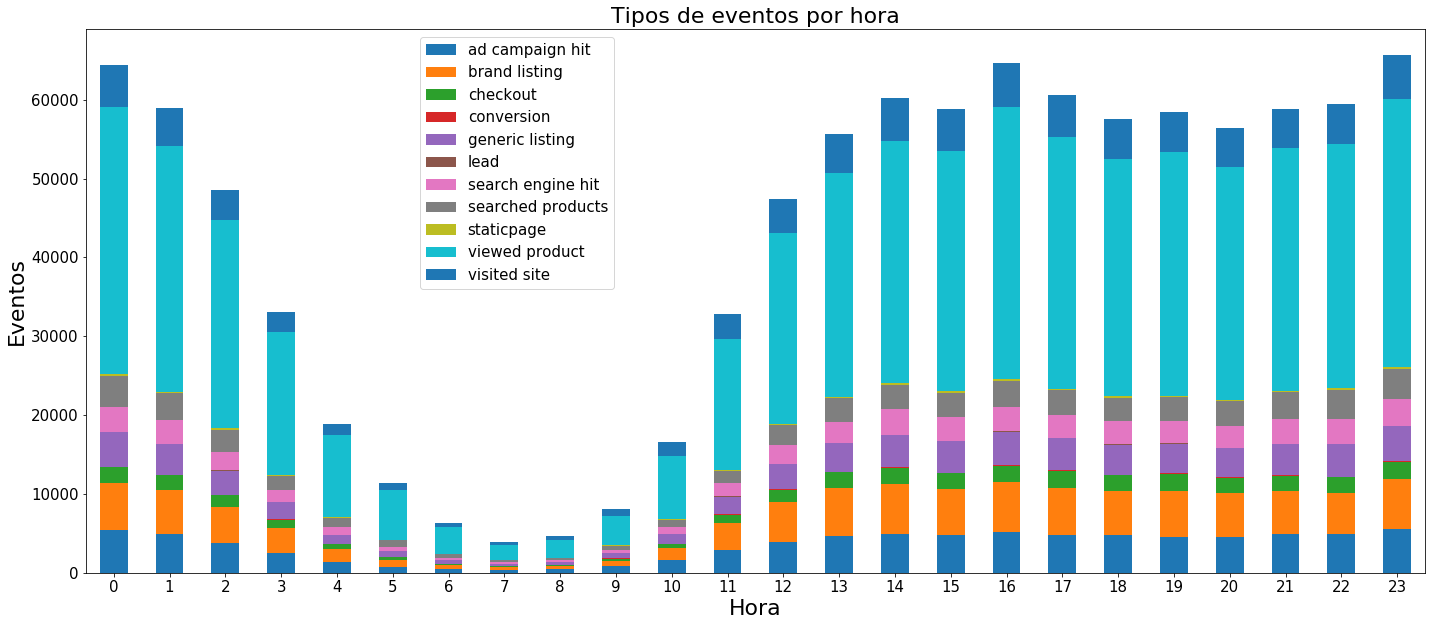
\includegraphics[width=1.1\linewidth]{output_12_1}
Figura 1.
\end{center}
	

Como se observa, a partir de las 01:00 hay una reducción importante en la cantidad de eventos, los cuales entre las 14:00 y las 00:00 se mantienen casi constantes y en valores altos.\\
 
\framebox[1.1\width]{La hora del día con más eventos es entre las 22:00 y las 23:00}  \\


Adicionalmente, este gráfico de barras apiladas evidencia el predominio de \textbf{"viewed product"} frente al resto de los eventos, siendo de aproximadamente un orden de magnitud mayor al evento que lo sigue en cantidad, podríamos filtrar a dicho evento para poder apreciar mejor la relación de los demás.\\

\begin{center}
	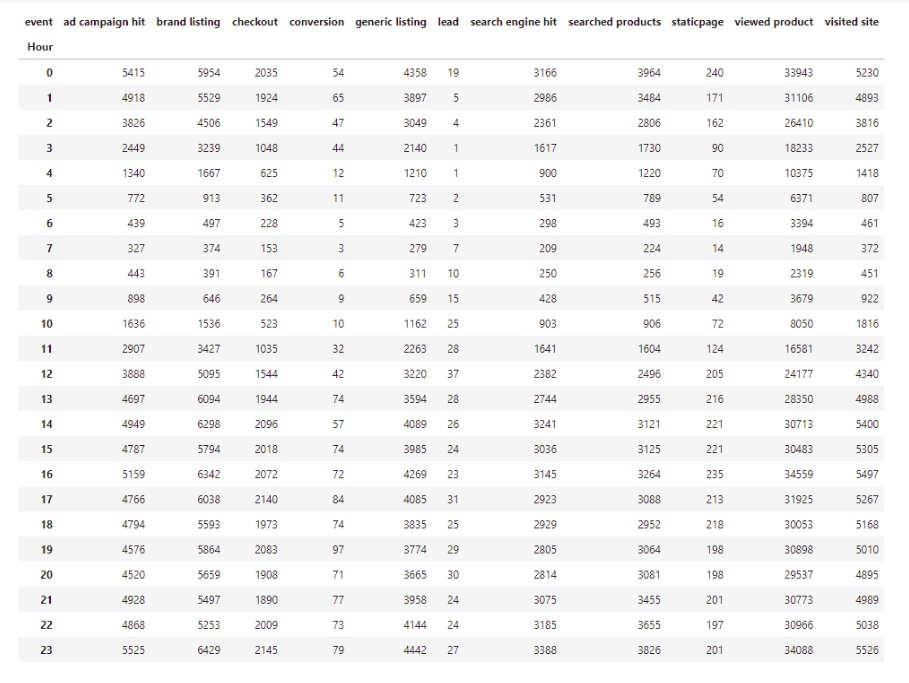
\includegraphics[width=1.1\linewidth]{table_1}
	Tabla 1: Tabla de frecuencias de eventos por hora

\end{center}

En el siguiente gráfico se pueden apreciar mejor las similitudes entre algunos eventos.
Mostramos un gráfico ilustrando algunos de los eventos de mayor ocurrencia durante el día (excluyendo a \textbf{"viewed product"}).\\
\begin{center}
	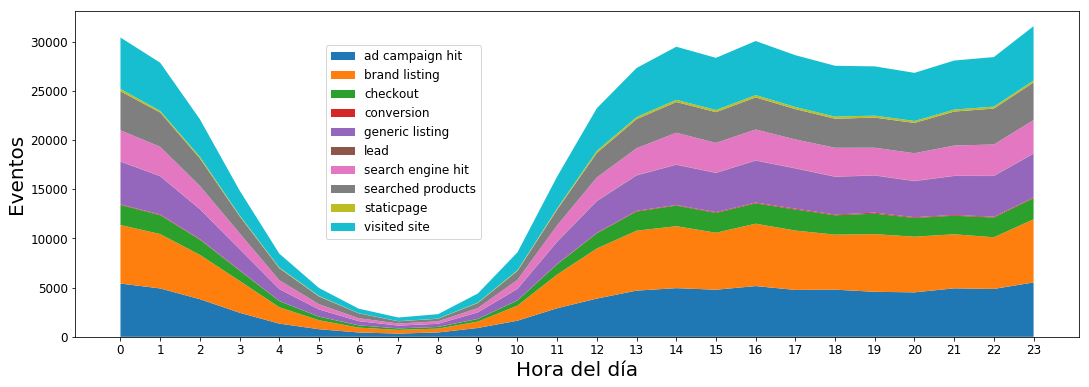
\includegraphics[width=1.1\linewidth]{output_16_0}
	Figura 2.
\end{center}

En el gráfico se aprecian los diferentes eventos de búsqueda, pudiendo ver una similitud en su tendencia temporal.

\begin{center}
	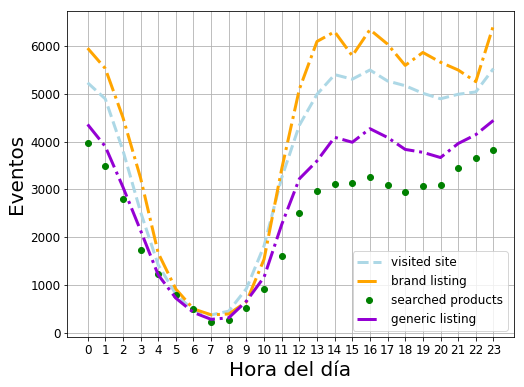
\includegraphics[width=1.1\linewidth]{output_18_0}
Figura 3.
	
\end{center}

\subsection{Evolución de la cantidad de eventos a lo largo del mes}
Se presenta un gráfico con la cantidad de eventos por día del mes:

\begin{center}
	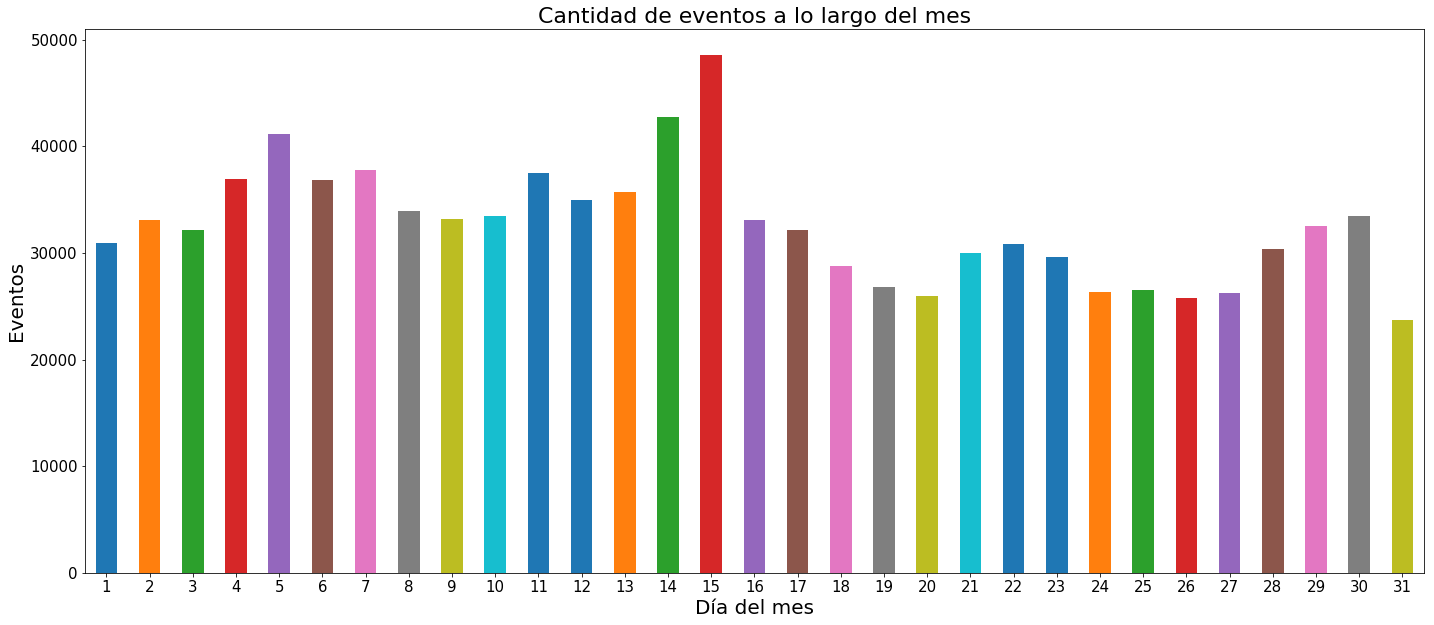
\includegraphics[width=1.1\linewidth]{output_21_1}
	Figura 4.
	
\end{center}

Lo interesante del grafico es que el día de más eventos es el dia 15 (mitad de mes), y a partir de ahí hay un gran descenso en la cantidad de eventos. Se puede pensar que la gente al cobrar a principio de mes, tiende a gastar más en la primer quincena.

\newpage
\subsection{Distribución de compras por hora del día y día del mes}
Continuando con el análisis temporal, se realizó un Heatmap para evidenciar la distribución de eventos durante el mes.

\begin{center}
	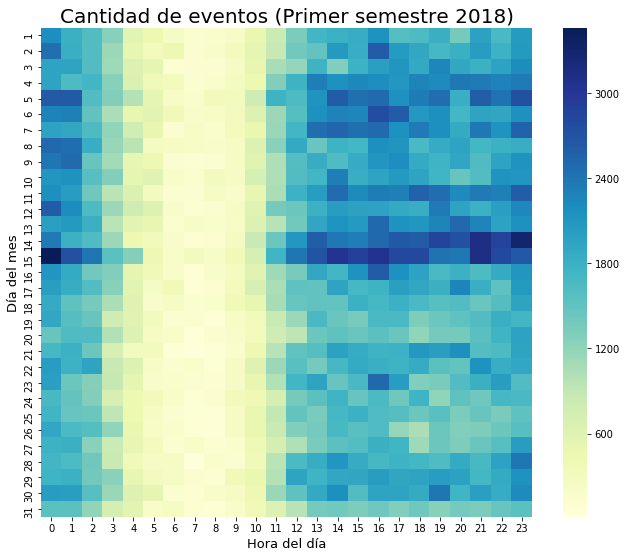
\includegraphics[width=1.1\linewidth]{output_24_1}
	Figura 5.
	
	\end{center}

Se puede observar un descenso en la cantidad de eventos en las horas de la mañana y un incremento particularmente interesante en los días 14 y 15 del mes, lo cual podría ser de utilidad a la hora de elegir la fecha para las ofertas o promociones mensuales.

\subsection{Distribución de eventos por día de la semana}

A continuación, se analizarán qué días de la semana tienen más eventos.

\begin{center}
	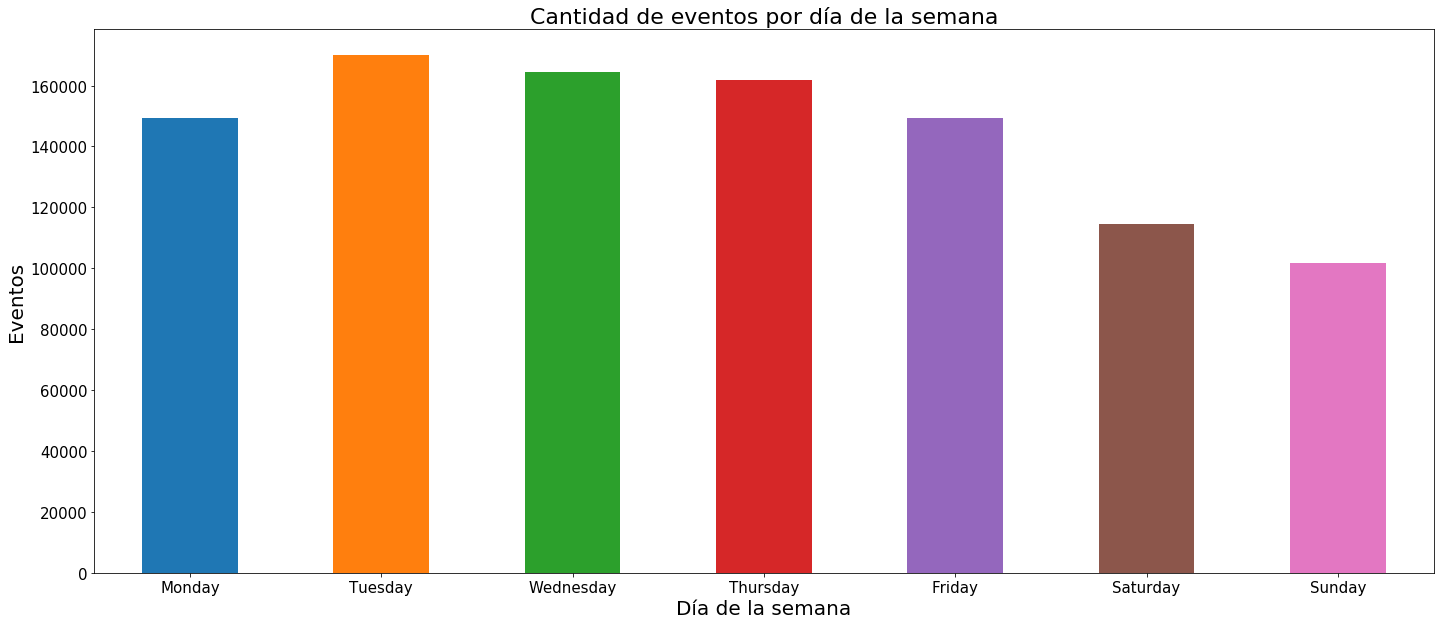
\includegraphics[width=1.1\linewidth]{output_27_1}
	Figura 6.
	
\end{center}

Se observa que el día martes es el más ocupado, y a partir de ahí se reduce gradualmente la cantidad de eventos, para luego aumentar nuevamente el lunes. \\

Es de destacar que los fines de semana hay muy poca actividad en relación con los demás días.\\

\begin{center}
	
\framebox[1.1\width]{El promedio de visitas de lunes a viernes es 158993}

\framebox[1.1\width]{El promedio en los fines de semana es 101709.}
\end{center}
\newpage

\subsection{Distribución de compras por día de la semana}
Continuando con el análisis de la sección anterior, se filtran los eventos que resultaron en compras (conversión).

\begin{center}
	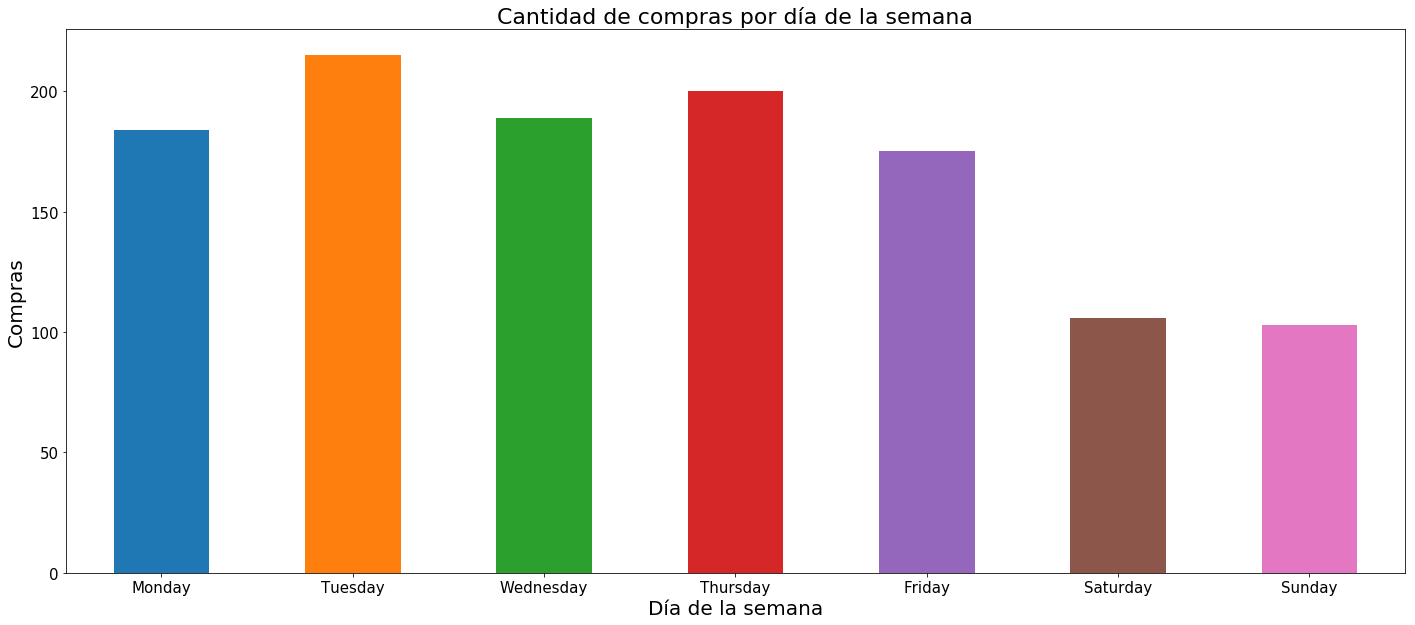
\includegraphics[width=1.1\linewidth]{output_31_1}
	Figura 7.
	
\end{center}

Se observa que la cantidad de compras mantiene la relación con la cantidad de eventos. \\

Es por esto que los martes son los días donde hubo más compras, mientras que en los fines de semana se registraron pocas compras.\\

\newpage
\subsection{Evolución de la cantidad de eventos a lo largo del año}	
Se procede a realizar un histograma mostrando la evolución en la cantidad de eventos a lo largo del año.

\begin{center}
	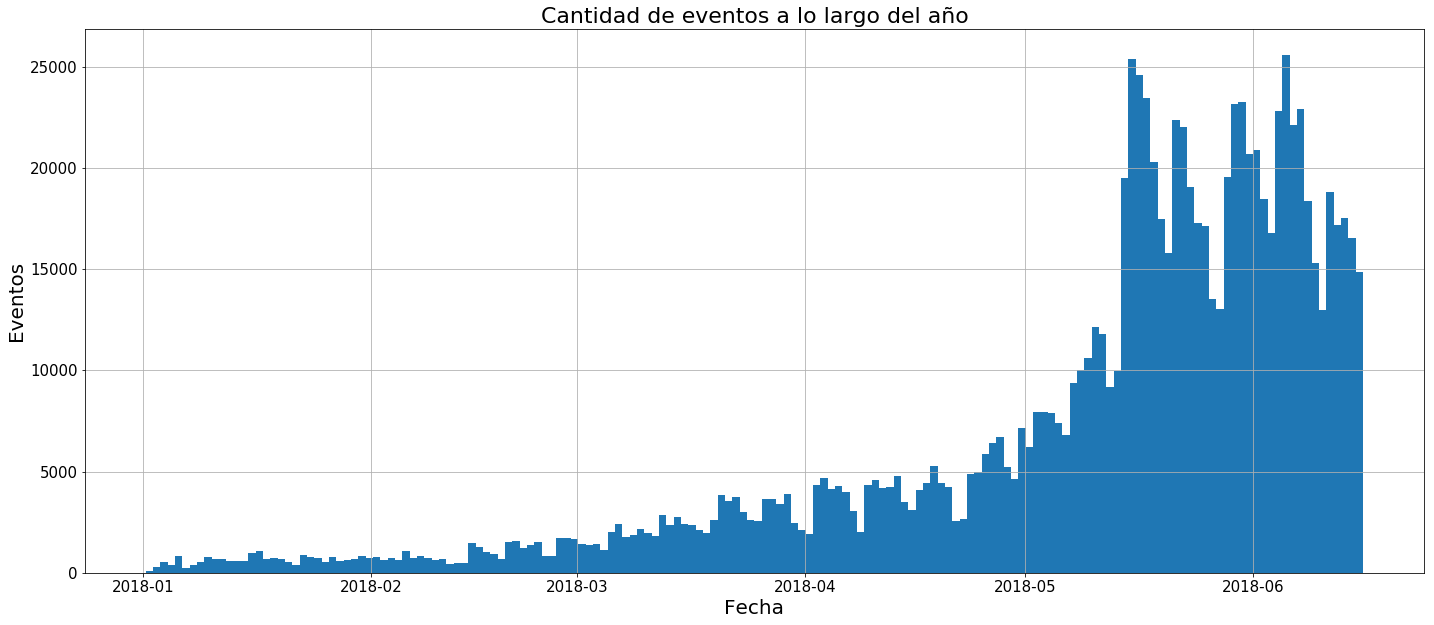
\includegraphics[width=1.1\linewidth]{output_34_1}
	Figura 8.
	
\end{center}

A partir del gráfico se deduce que, o bien los primeros 4 meses no hubo una cantidad significativa de eventos, o estos no fueron registrados.\\

 Igualmente, en los meses de mayo y junio se observa un gran incremento en la cantidad de eventos, con un gran salto a mitad del mes de mayo.\\
 
  Se necesitarán más datos para predecir el progreso en los futuros meses, pero parece indicar que se mantendrán constantes la cantidad de eventos.

\newpage  
\subsection{ Evolución de la cantidad de compras a lo largo del año}

Se muestra un histograma de las compras a lo largo del año:

\begin{center}
	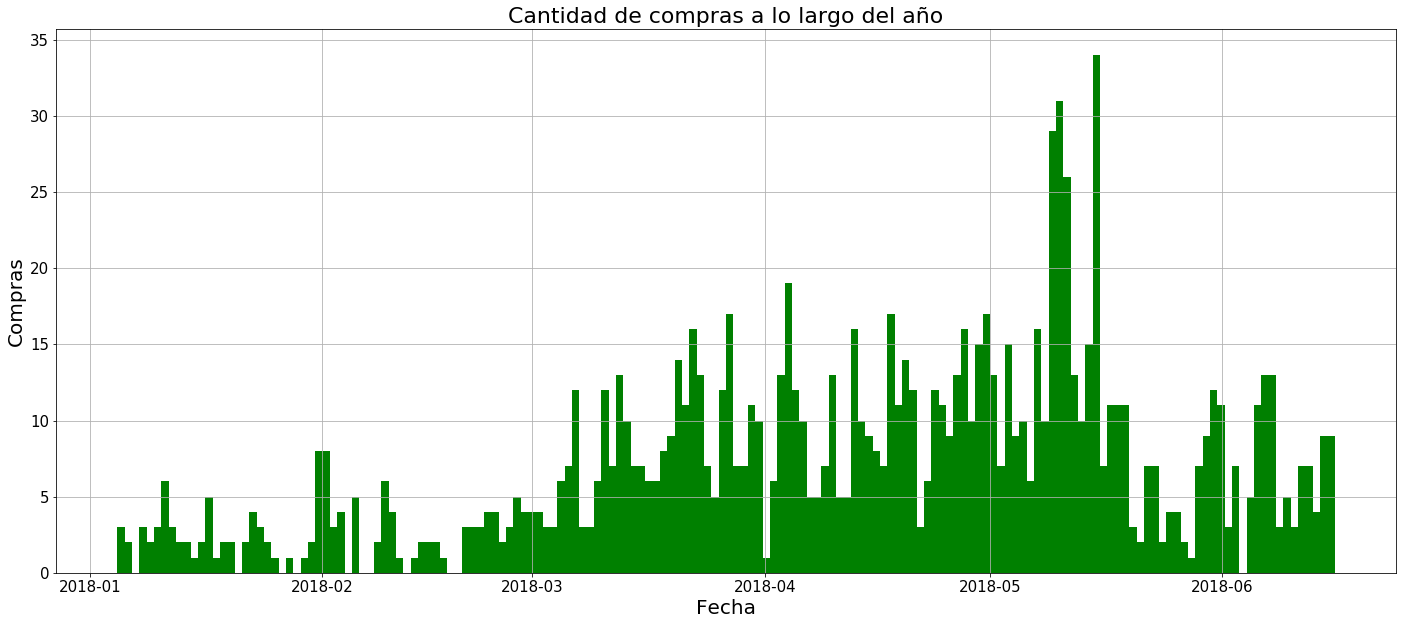
\includegraphics[width=1.1\linewidth]{output_37_1}
	Figura 9.
	
\end{center}

Filtrando por compras, se observa que a partir del mes aumentaron lentamente, manteniendo un umbral de 20 compras diarias.\\

 Sin embargo, a mitad del mes de mayo hubo picos de compras, durante 3 días seguidos se vendieron más de 25 celulares por día (tal vez debido a una promoción). \\
 
 En los últimos días, se volvió a los niveles anteriores (menores a 20 compras diarias), tal vez indicando la necesidad de una nueva promoción.\\

\begin{center}
	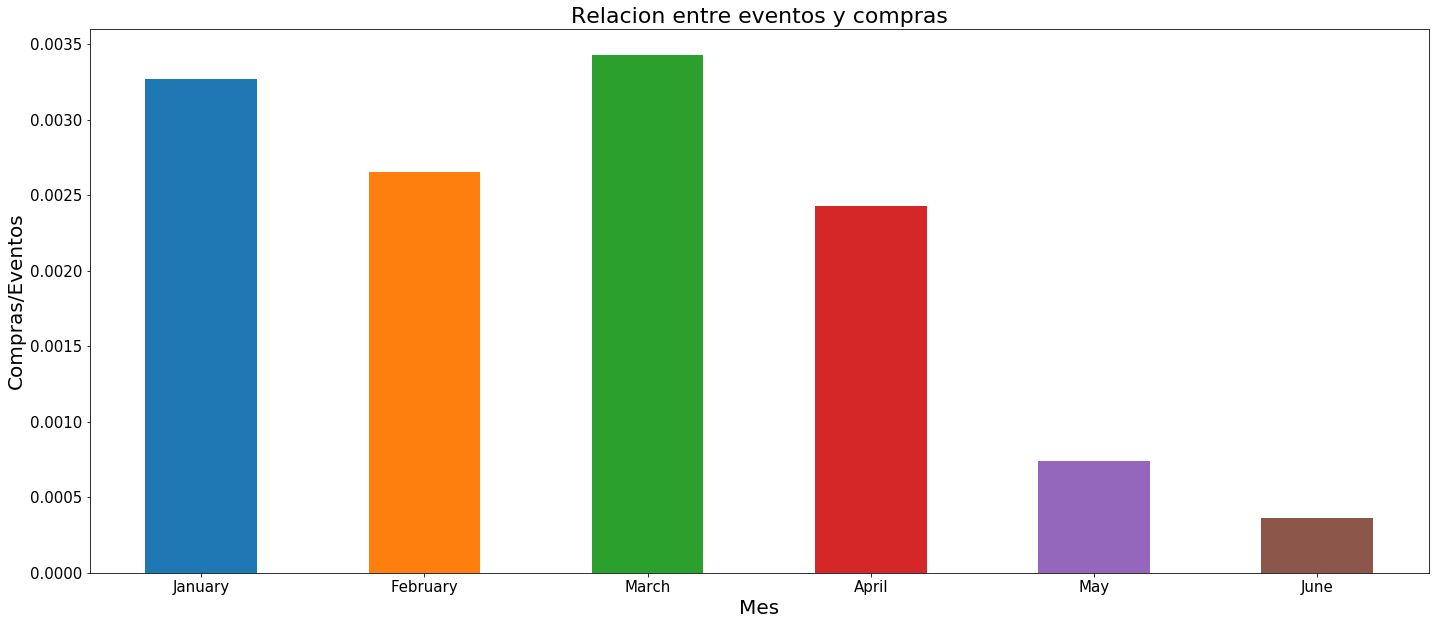
\includegraphics[width=1.1\linewidth]{output_39_1}
	Figura 10.
	
\end{center}

En este gráfico observamos que si bien las visitas aumentaron en los últimos meses, las compras no lo hicieron con la misma intensidad, y por lo tanto, la relación entre eventos y compras fue disminuyendo.\\

\begin{center}
	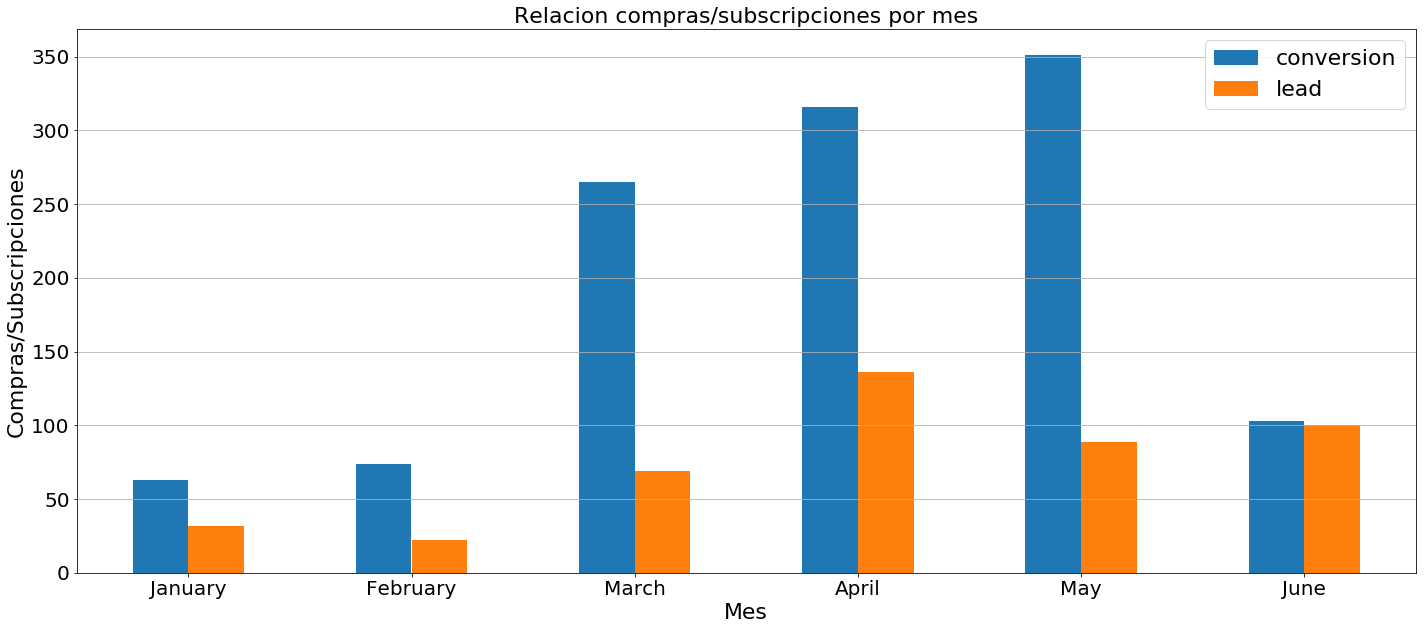
\includegraphics[width=1.1\linewidth]{output_41_0}
	Figura 11.
	
\end{center}

Por otro lado, aunque las compras aumentan lentamente mes a mes, las subscripciones no mantienen una tendencia fija, variando mes a mes. \\

Un dato interesante es que en lo que va del mes de junio, prácticamente todas \textbf{las compras provocaron subscripciones nuevas}, lo cual indica que hubo una mejora en ese aspecto.

\subsection{Usuarios nuevos}

\begin{center}
	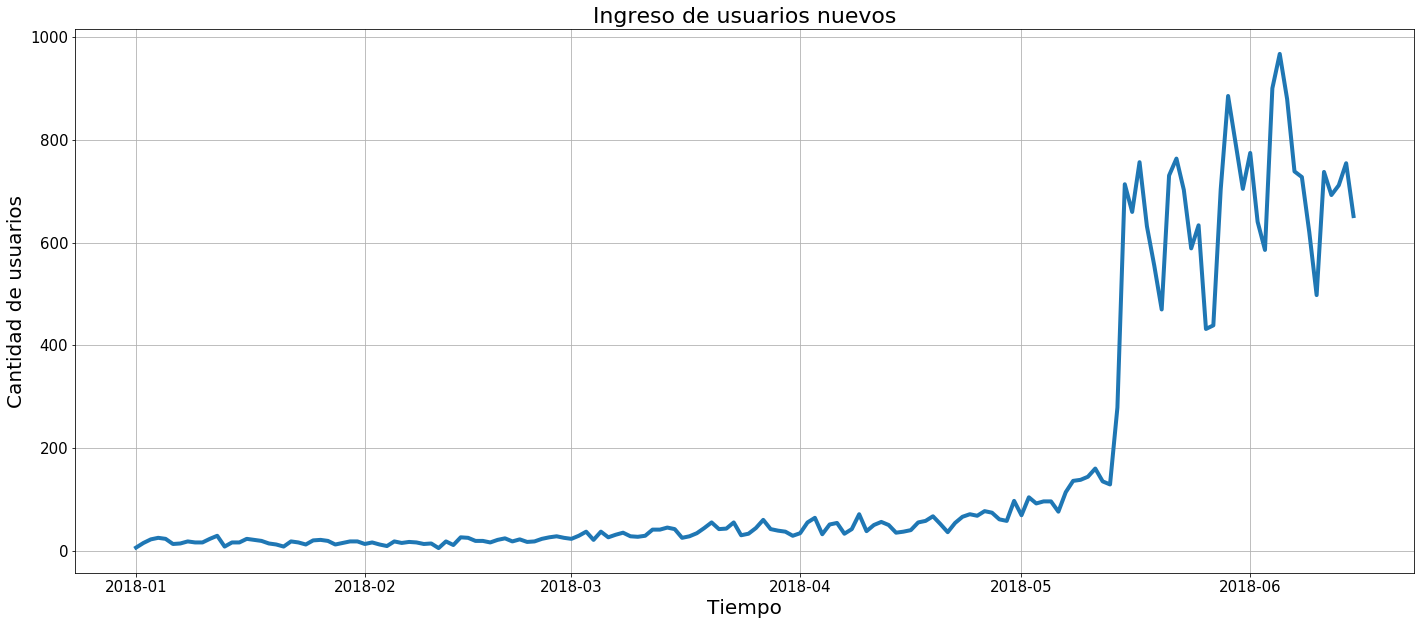
\includegraphics[width=1.1\linewidth]{output_44_0}
	Figura 12.
	
\end{center}

Durante los primeros 4 meses, la cantidad de usuarios nuevos se mantuvo constante, por debajo de las 100 personas, pero a mediados de mayo, hubo un gran aumento repentino, que se mantuvo constante durante las ultimas semanas, y por lo que se observa, al haber picos cada vez mayores, la tendencia es alcista.



\newpage

\section{Análisis de eventos}

A continuación, vamos a analizar cuáles son los eventos más importantes y a partir de ello, ver cómo se relacionan con los demás datos y entre ellos, ya sea la cantidad de eventos que una persona genera, el tipo de los mismos, la cantidad de eventos promedio antes de una “conversion”.\\


Debido a que la cantidad de clases de evento es de once, un número con el que no habrá problemas en el procesamiento de los mismos y las visualizaciones se decidió trabajar con la totalidad de estos.\\


Esto nos brinda un panorama general frente a los análisis y nos ahorra el descarte de información que podría ser de utilidad. 


\subsection{Cantidad de eventos por usuario}

En un primer análisis, buscamos tener un panorama general sobre el comportamiento de los usuarios en el sitio. Para eso, agrupando por usuario, y teniendo en cuenta todos los eventos, tenemos la cantidad de eventos que cada uno generó.\\


Cabe aclarar que el análisis consecuente se hará con una muestra de 27624 usuarios, que generaron un total de 1011288 eventos.\\


Una mirada rápida de este set de datos nos permite obtener las siguientes características:


\begin{center}
	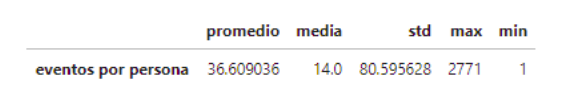
\includegraphics[width=0.8\linewidth]{table_2}\\
	Tabla 2: Características de eventos por persona.
	
\end{center}



Veamos que la media de la cantidad de eventos generados por usuario es de 14, teniendo un desvío estándar de aproximadamente 80, esto indica la variabilidad considerable que posee nuestra muestra, y nos da un primer indicio de que podría ser conveniente no analizar la totalidad de los usuarios, sino un subconjunto de estos.\\


Veamos que, pese a que la media es de 14 eventos por usuario, nuestro valor máximo es de 2771, lo que nos advierte que nuestra muestra podría contener outliers, es decir, usuarios (en general en poca cantidad) que generan una cantidad de eventos que no obedecen a los estimadores de nuestra muestra, particularmete en nuestro caso, se trata de usuarios que generan una gran cantidad de eventos.\\


Por ultimo pero no menos importante, una moda de 4 eventos, con un valor de 3248 usuarios nos sugiere una distribución muestral sesgada hacia la izquierda.
Pese a que nuestro valor máximo es de 2771, si graficamos la cantidad de usuarios por eventos generados obtenemos:\\

\begin{center}
	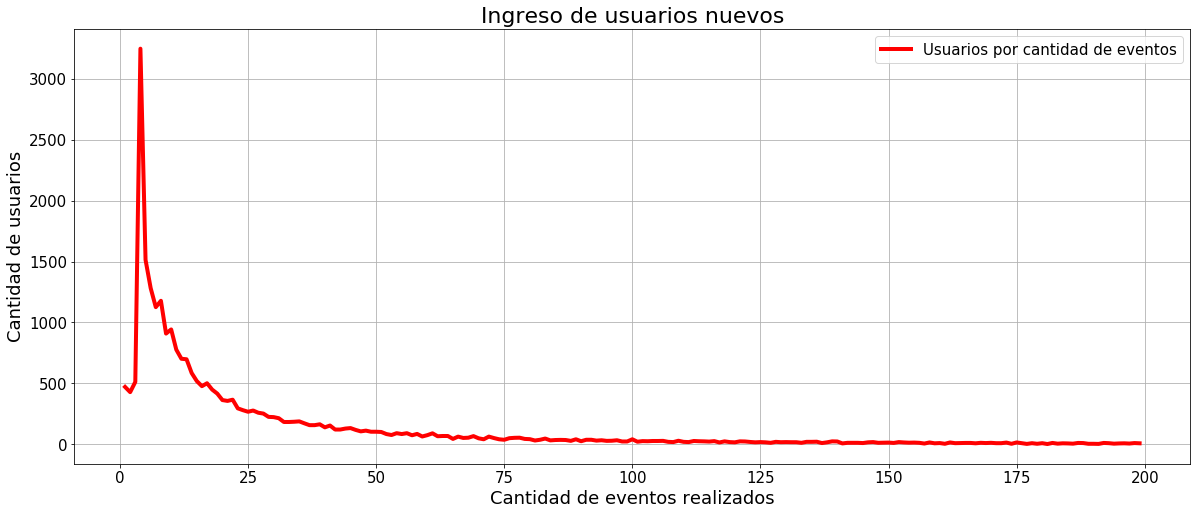
\includegraphics[width=1.1\linewidth]{output_52_0}
	Figura 13.
	
\end{center}

Por motivos de visualización, y al observar que la muestra es decreciente, decidimos no graficar la totalidad del soporte, ya que la zona con mas cantidad de usuarios sería demasiado estrecha para sacar conclusiones.\\


Elegimos en particular el primer decimo del mismo, que ya de por si nos esclarece las suposiciones previas que habíamos tenido en cuenta.\\


En particular, se observa una clara disminución en el número de usuarios con más de 75 eventos. Esto nos indica que la cantidad de usuarios con más eventos, va a ser despreciable frente al resto (en particular del orden de las centenas para valores menores a 25 eventos)\\

\newpage

Este grafico de línea nos sugiere desestimar dichos valores. Para poder tener una mejor observación de la muestra. 
Una vez realizado el filter, se presentan dos violin plots que facilitan nos presentan de forma visual una idea más precisa de nuestra muestra. 
\\

\begin{center}
	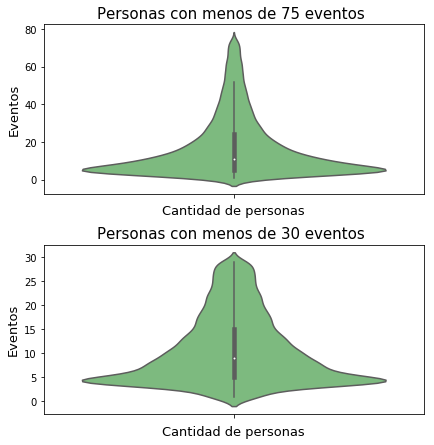
\includegraphics[width=1.1\linewidth]{output_55_1}
	Figura 14.
	
\end{center}

Se filtraron correspondientemente las personas con mas de 75 y 30 eventos. Se eligieron estos valores meramente con fines visuales.\\


En el primer caso, por la poca cantidad de valores superiores a dicho rango (obteniendo un intervalo aproximadamente hasta: media + std )\\


En el segundo caso se busco principalmente presentar un intervalo de valores simétricos con respecto a la media.\\


En el interior de cada plot se ve la distribucion de los valores y su media.\\



\subsection{Eventos generados por usuarios}
De ahora en adelante tendremos en cuenta los tipos de eventos generados por dichos usuarios y su correlación, con el fin de detectar cualquier tipo de similitud o patrón de los mismos.\\


A continuación, presentamos un gráfico de barras con los distintos eventos y la frecuencia absoluta de los mismos:

\begin{center}
	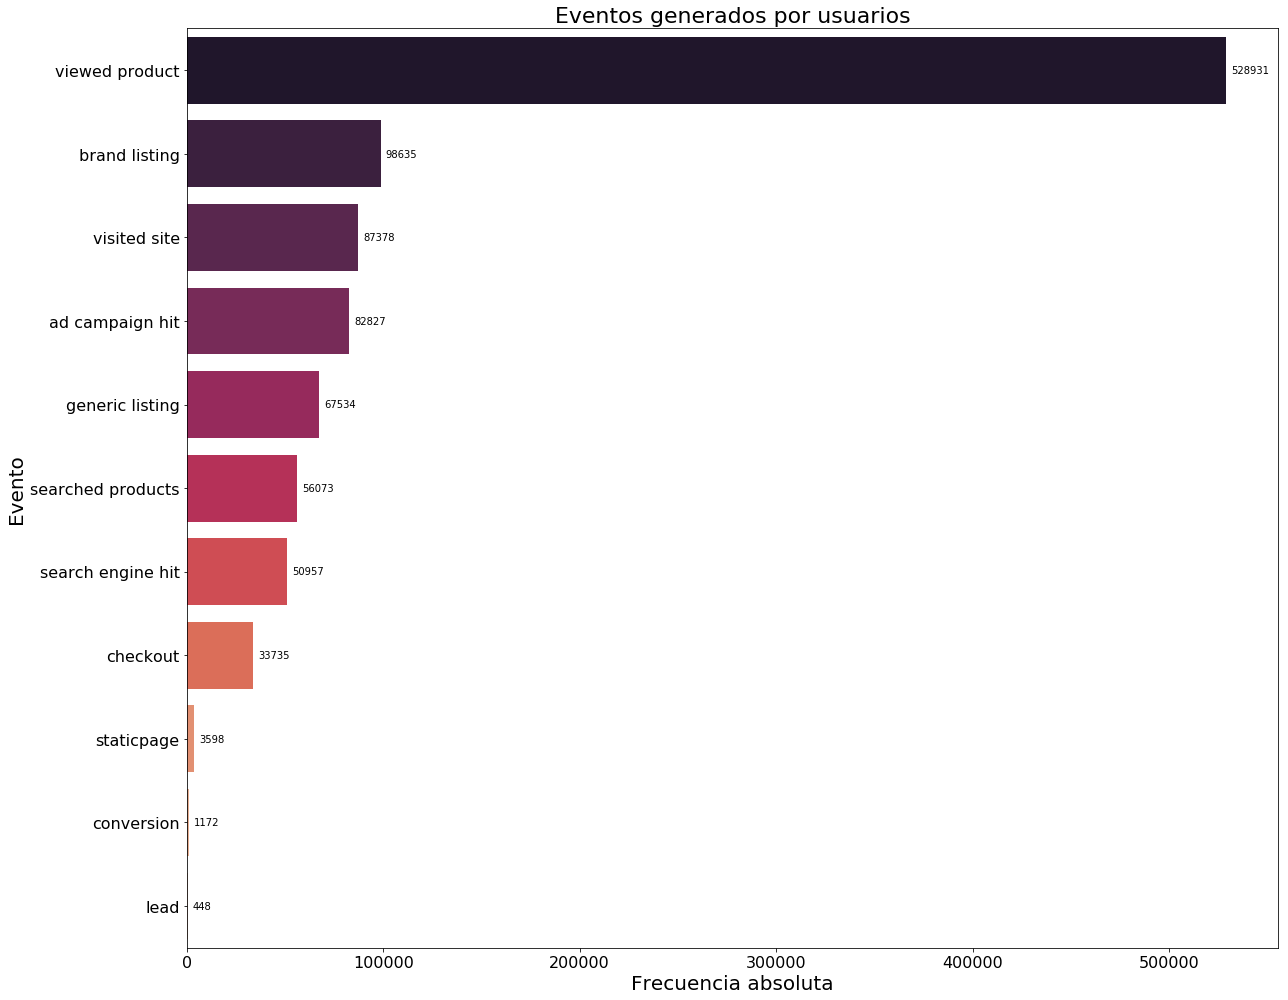
\includegraphics[width=1.0\linewidth]{output_58_0}
	Figura 15.
	
\end{center}
Se puede observar una dominación absoluta del evento “viewed product”, debido a que muchos de los demás eventos se generan junto con el mismo en una secuencia de eventos.\\


\emph{
Algo que parece importante destacar es que solamente el 3\% de las veces que se ingresa al “checkout” se termina realizando una “conversion”, es decir, efectuando una compra.\\}


Esto podría deberse, entre otros, a estos \underline{dos factores}:

\begin{itemize}
	\item El proceso de “checkout” no transmite la seguridad necesaria.
	
	\item El proceso desde “checkout” hasta “conversión” es excesivamente complejo.
	
\end{itemize} 

\subsection{Modelos más vendidos}


A continuación se presenta una lista con los modelos más vendidos, la información que se extrae de la misma podía ser de utilidad para reforzar las ofertas y publicidades sobre estos modelos, y disminuir a aquellos en los cuales no se están produciendo una cantidad considerable de ventas.\\

\begin{center}
	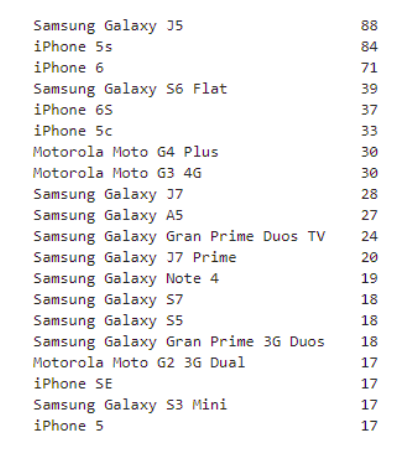
\includegraphics[width=0.6\linewidth]{table_3}
	\\Tabla 3: Modelos más vendidos.
	
\end{center}

En un primer análisis general, se observa que celulares de gama media son los más frecuentes, destacando la tendencia a los modelos de Samsung, Apple y Motorola.\\


Solo acercamos una conclusión rápida por el momento, ya que el análisis con respecto a las Marcas se realizara en otra sección con más profundidad.\\



Otra observación es que en el Top-3 de modelos vendidos, los valores presentan una gran similitud. En contraste a la relación con sus relegados seguidores, cuyas ventas son menores que la mitad de las de estos.\\

Como complemento visual a la presentación de tabla, se incluye un gráfico de barras de dicho set:\\

\begin{center}
	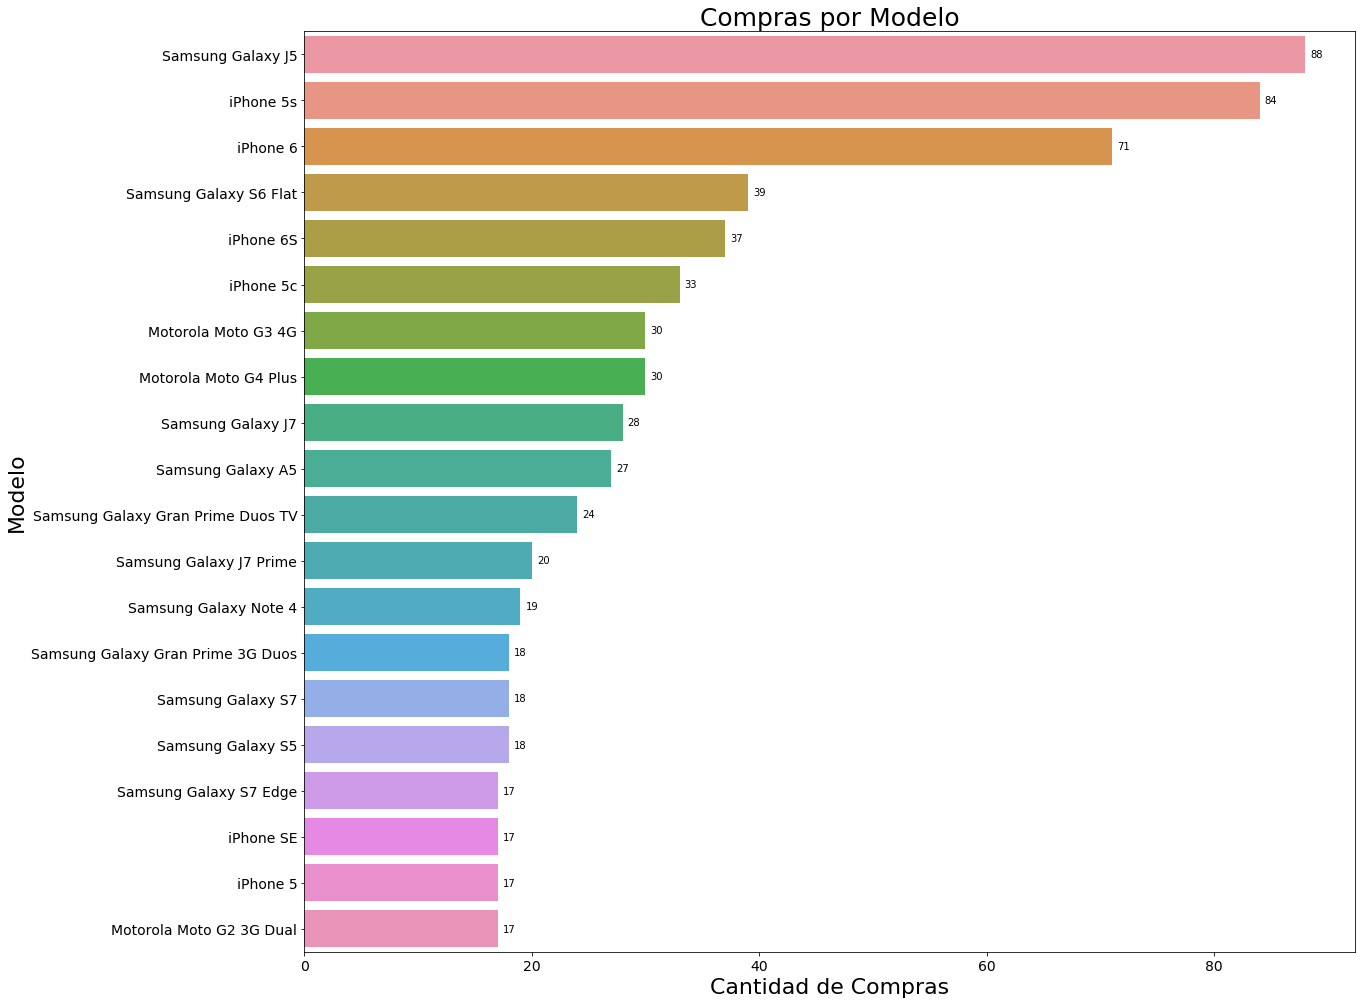
\includegraphics[width=1.1\linewidth]{output_61_0}
	Figura 16.
	
\end{center}
\newpage
Adentrándonos en la observación rápida sobre las ventas por marcas, se presenta un gráfico con la cantidad de ventas por marca: \\

\begin{center}
	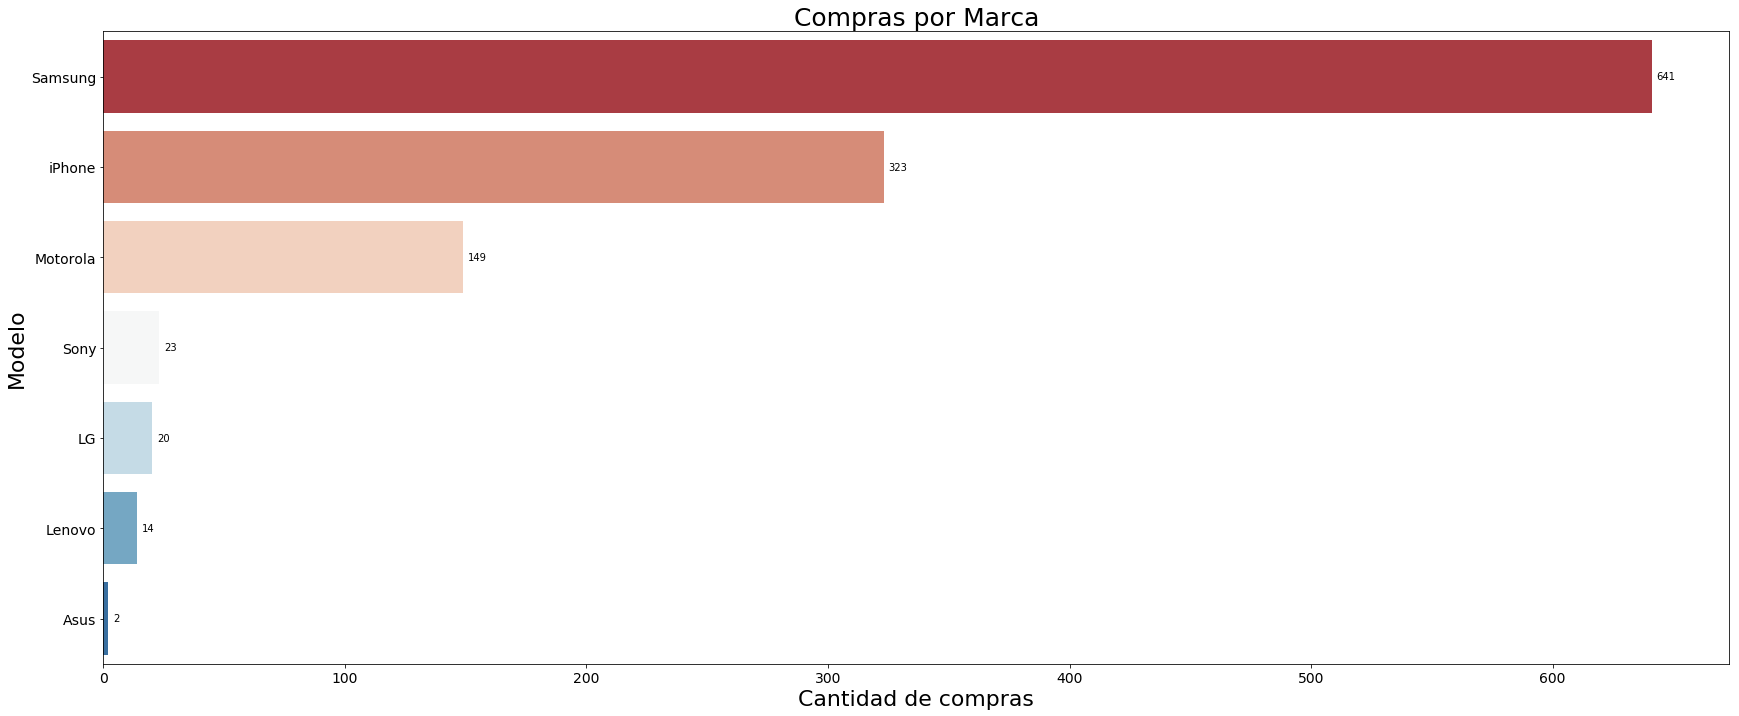
\includegraphics[width=1.1\linewidth]{output_63_0}
	Figura 17.
	
\end{center}

El gráfico reafirma las conclusiones previas situando a Samsung, Apple (iPhone) y Motorola como los lideres en este rubro. \\

Adicionalmente el gráfico nos permite ver la supremacía de dichas marcas con respecto a sus competidoras, cuyos ordenes de ventas son como a lo sumo un 10\% de las lideres.


Otro aspecto importante para analizar es la cantidad de visitas por marca, lo cual, en conjunto con el gráfico previo, puede evidenciar la tendencia que tienen los usuarios al considerar una marca en particular, pero luego no realizar la compra.\\

\begin{center}
	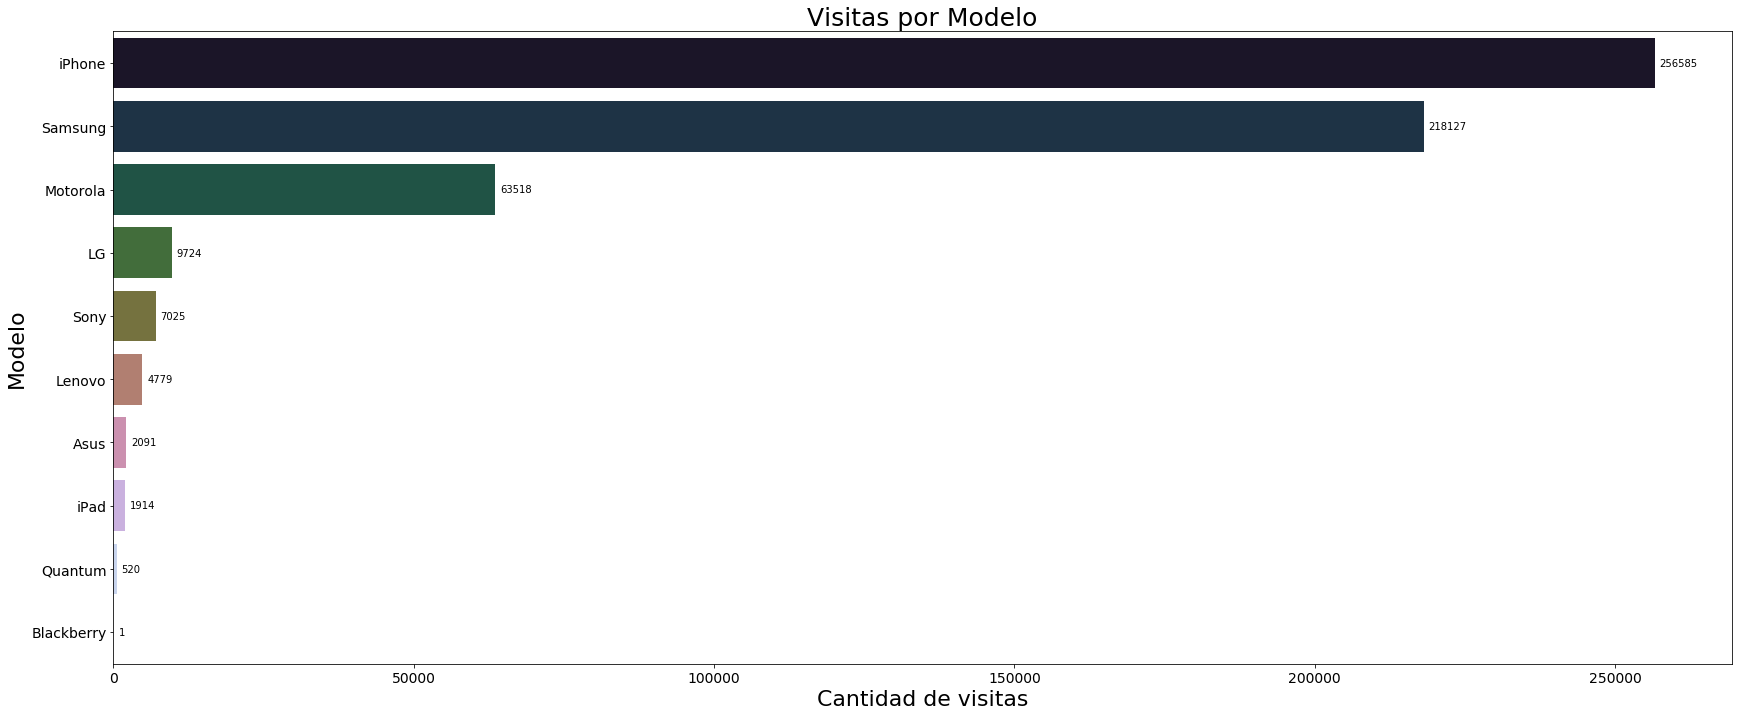
\includegraphics[width=1.1\linewidth]{output_65_0}
	Figura 18.
	
\end{center}

Se puede observar que los celulares iPhone son altamente visitados, pero luego el rango de compra disminuye de forma mas abruptamente que las marcas Samsung y Motorola, a continuación se presentan la razón entre la cantidad de ventas y visitas por marca:
\begin{itemize}
	\item \textbf{iPhone}: 794.380805
	\item \textbf{Samsung}: 340.603744
	\item \textbf{Motorola}: 426.29530 
\end{itemize}

Teniendo en cuenta dicha razón, se puede concluir que los usuarios que visitan modelos Samsung tienen mayor tendencia a comprar que las demás marcas.\\


Cabe aclarar que no se consideraron las demás marcas debido a la baja cantidad de ventas de estas con respecto a las tres mencionadas, evitando caer en un mal uso de la ecuación de de-Moivre, y en conclusiones erróneas. 
\\


Para continuar el análisis de estas tres marcas se propone observar la evolución de sus ventas a lo largo de los meses, con el fin de observar tendencias en las mismas:\\

\begin{center}
	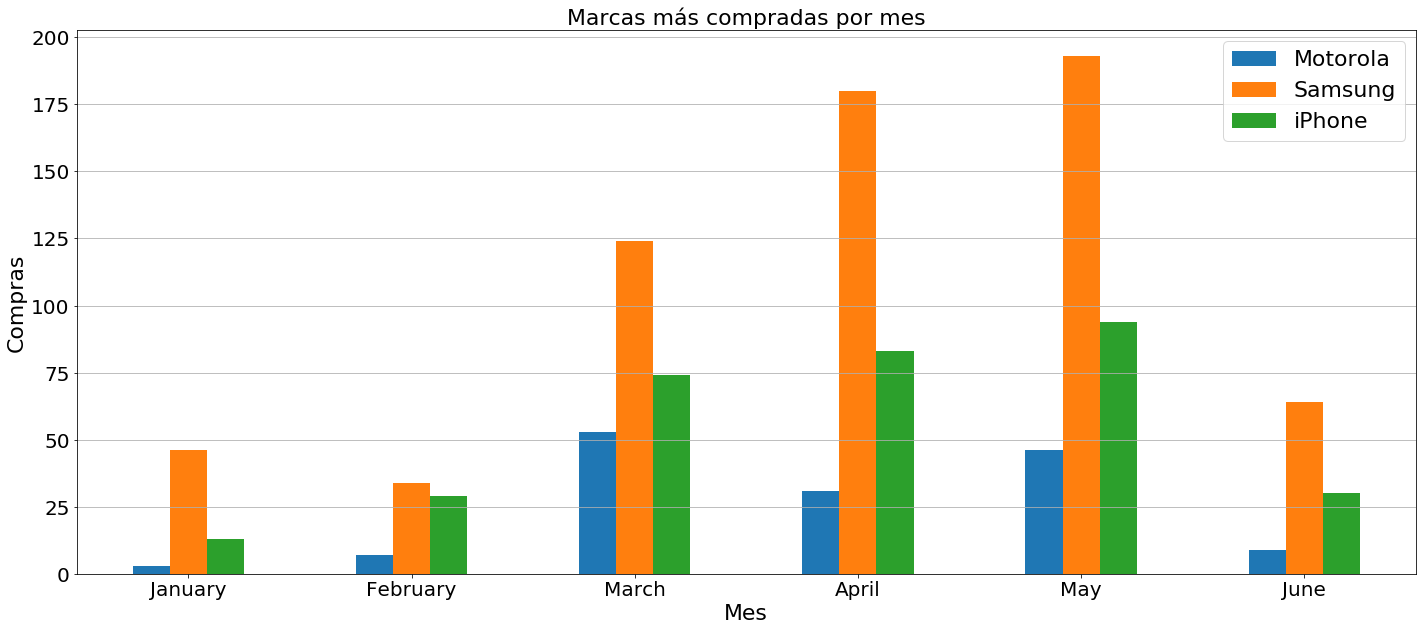
\includegraphics[width=1.1\linewidth]{output_67_0}
	Figura 19.
	
\end{center}

Se puede observar un crecimiento paulatino en las marcas Samsung y Apple(iPhone) en los primeros cinco meses del año. Una explicación para la disminución de las ventas en enero, febrero y junio podría ser la falta de promociones y difusión del sitio, o el lanzamiento de nuevos modelos en los meses con mas ventas.\\


Se ve un comportamiento errático de la marca Motorola, en torno a las 25 ventas por mes.\\

\subsection{Capacidad de los equipos}
Otro aspecto relevante es la Capacidad de los equipos, es conocida la tendencia al aumento de la misma en los nuevos modelos, debido a aumentos en los tamaños de las actualizaciones y Sistema Operativo y mayor flujo de multimedia a almacenar.\\


Usualmente, las capacidades de 16GB y 32GB son las más solicitadas, debido a su comodidad y precio frente a otras mayores.\\

\newpage
Dicha tendencia se evidencia en el siguiente gráfico:

\begin{center}
	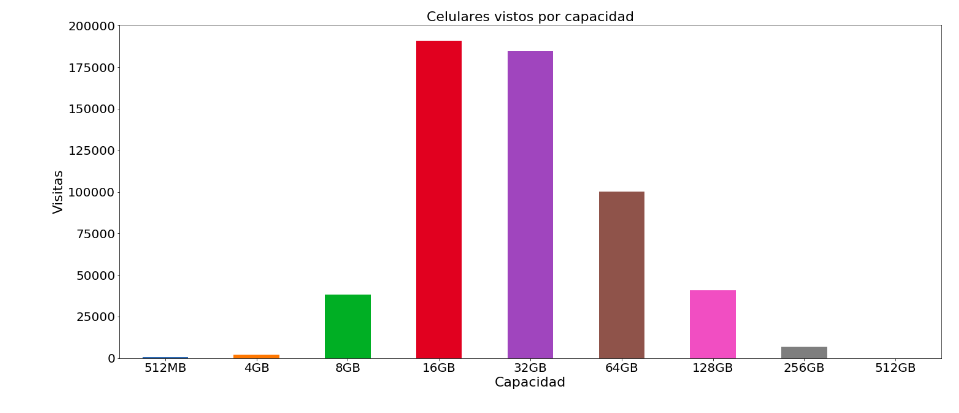
\includegraphics[width=1.1\linewidth]{output_69_1}
	Figura 20.
	
\end{center}

Si adicionamos al mismo el gráfico de Ventas por capacidad, se observa una moda en los celulares de 16GB, que posiblemente provenga a la armonía capacidad/precio que en la actualidad ofrecen.
\\

\begin{center}
	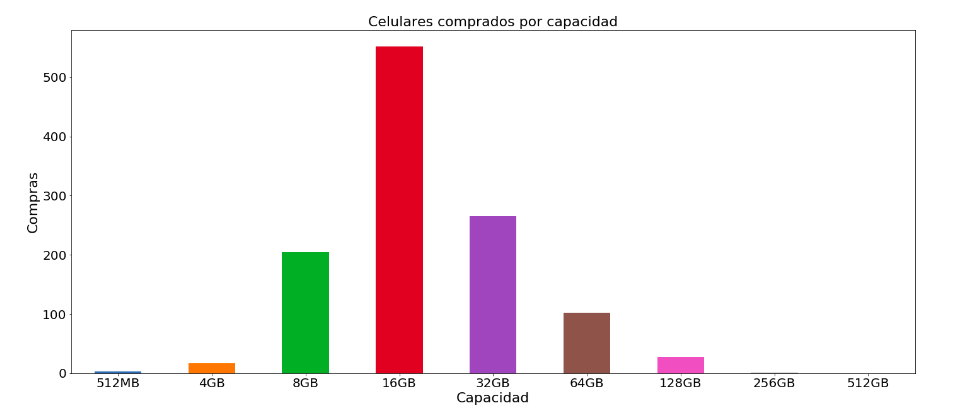
\includegraphics[width=1.2\linewidth]{output_70_1}
	Figura 21.
	
\end{center}

\subsection{Compras por condición}
Otra faceta interesante a presentar el las vistas de los celulares en función de su condición:
\begin{center}
	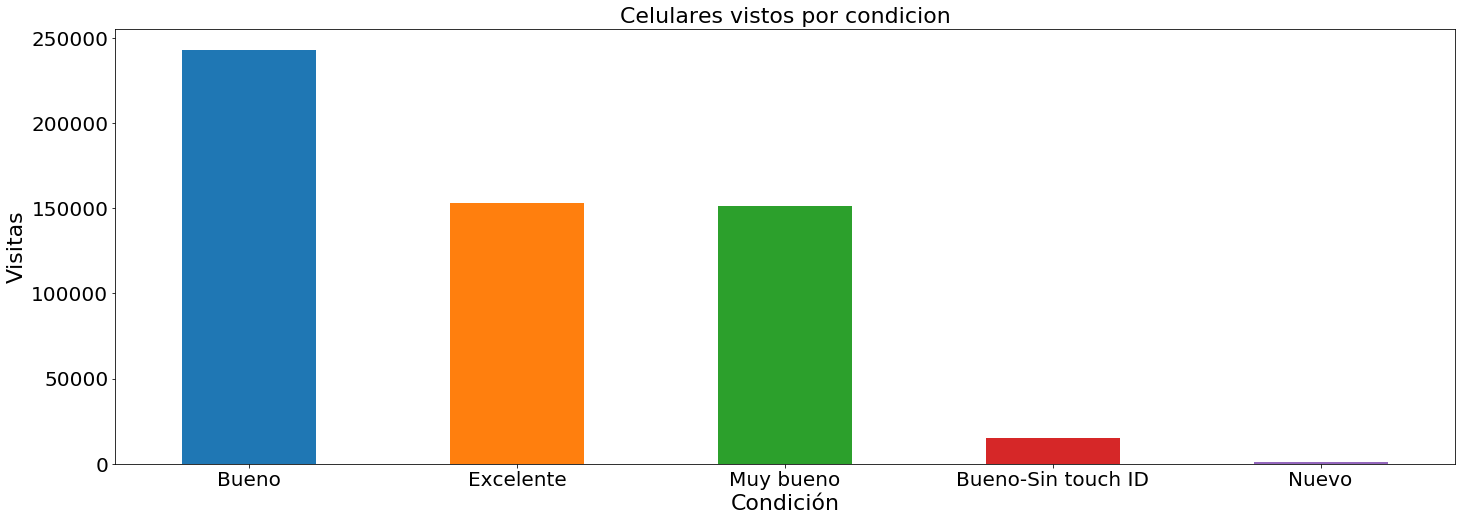
\includegraphics[width=1.1\linewidth]{output_72_1}
	Figura 22.
	
\end{center}

La desestimable cantidad de vistas en celulares nuevos remarca el espíritu del sitio, mientras que los celulares buenos son los más observados, posiblemente por una interesante disminución de su precio en un producto todavía funcional y duradero.\\


Si además, como en los anteriores análisis, agregamos un gráfico de compras, podremos ver la clara tendencia a celulares buenos, disminuyendo mientras mejor condición presentan los mismos:\\

\begin{center}
	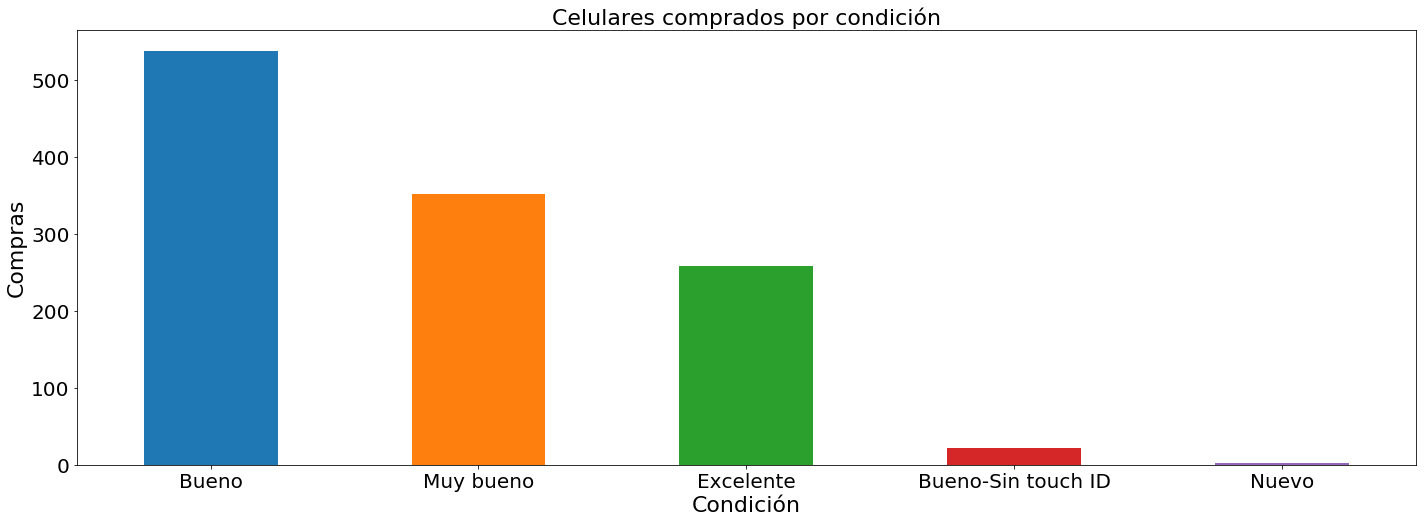
\includegraphics[width=1.1\linewidth]{output_73_1}
	Figura 23.
	
\end{center}

Adicionalmente, es de interés conocer el origen de los usuarios, en este gráfico se pretende exhibir la cantidad de usuarios provenientes de una campaña a lo largo de los meses del set:\\

\begin{center}
	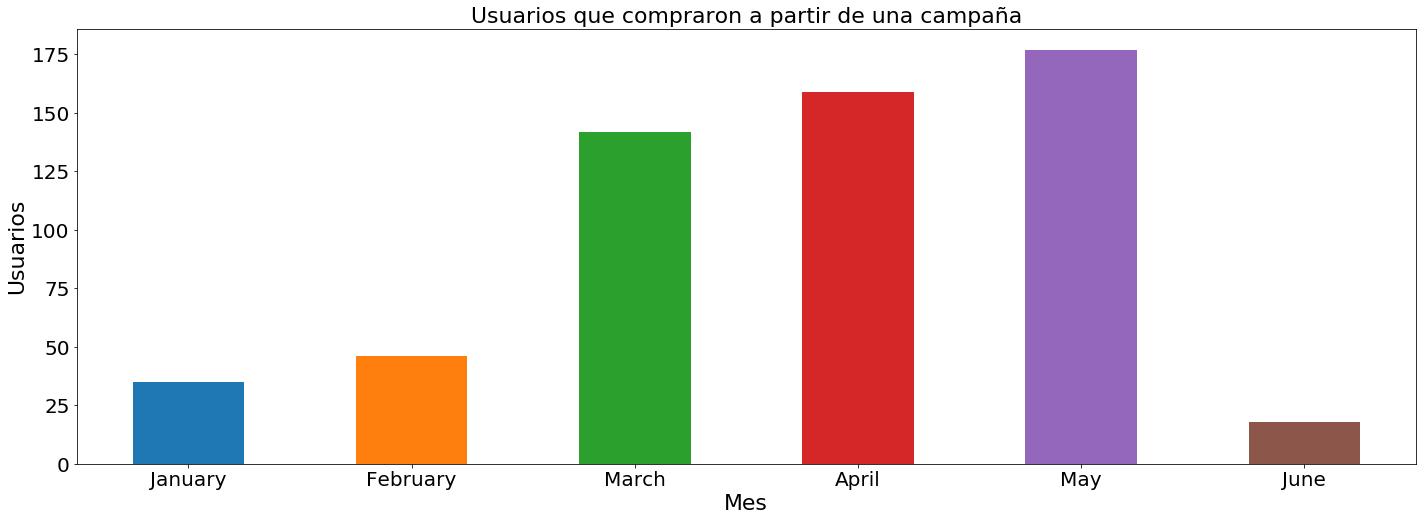
\includegraphics[width=1.1\linewidth]{output_75_1}
	Figura 24.
	
\end{center}

Esto podría relacionarse con la venta de equipos de las marcas líderes (Samsung, iPhone y Motorola), cuyos picos de venta ocurrieron en estos meses. 
El conjunto de ambos gráficos podría servir como una iniciativa para intentar incrementar los usuarios que provienen de campañas.\\
\newpage

\subsection{Cantidad de eventos por tipo de dispositivo}
En este párrafo nos centraremos a diferenciar los diferentes tipos de dispositivos y la cantidad de eventos en los que estuvieron involucrados:\\

\begin{center}
	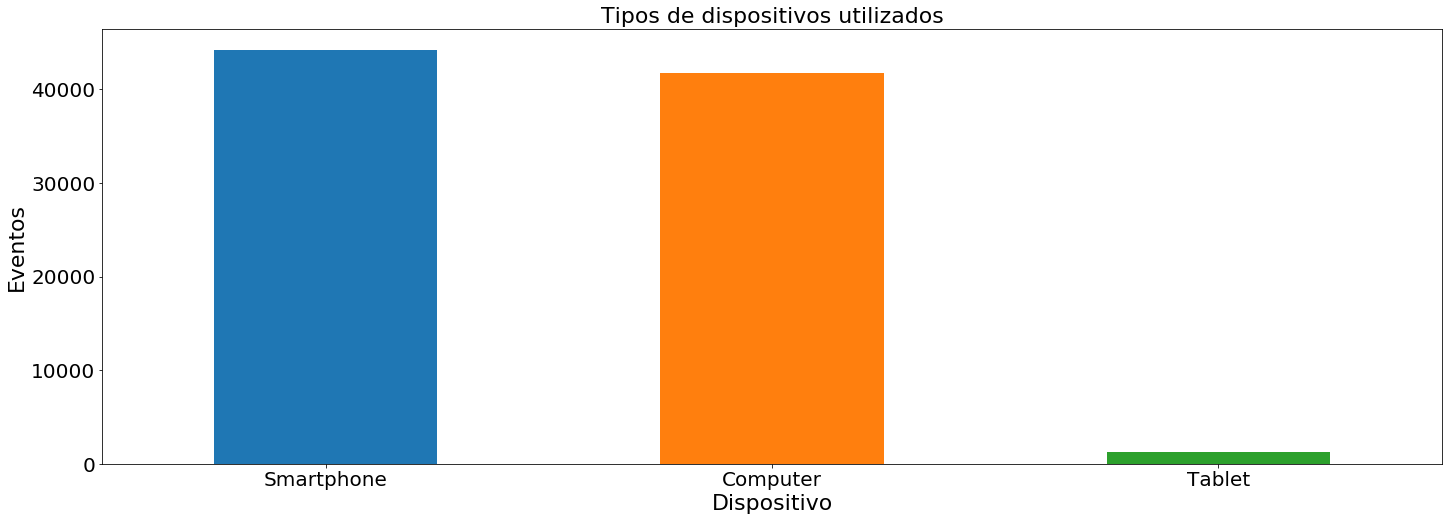
\includegraphics[width=1.1\linewidth]{output_78_1}
	Figura 24.
	
\end{center}


Se observa una tendencia marcada a la elección de Smartphones y Computadoras, siendo Tablet un tipo de dispositivo muy poco utilizado.
Esto puede deberse, entre otras cosas, a la poca reutilización del producto, la carencia de información de los usuarios de estos en el sitio, o la menor popularidad del mismo frente a los demás dispositivos.
\\


\subsection{Navegadores preferidos}


En esta sección se pretende hacer un análisis de los Navegadores Web más utilizados. Para comenzar se muestra una lista de los mismos, y un gráfico de barras que permite evidenciar mejor la relación entre los navegadores mas usados:\\

\begin{center}
	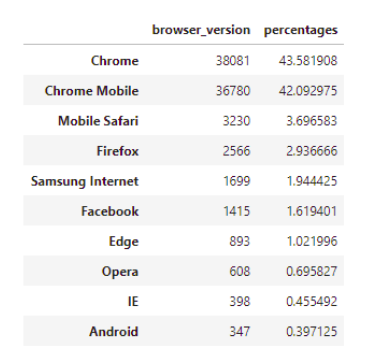
\includegraphics[width=0.7\linewidth]{table_4}
	\\Tabla 4: Navegadores preferidos.
	
\end{center}

\begin{center}
	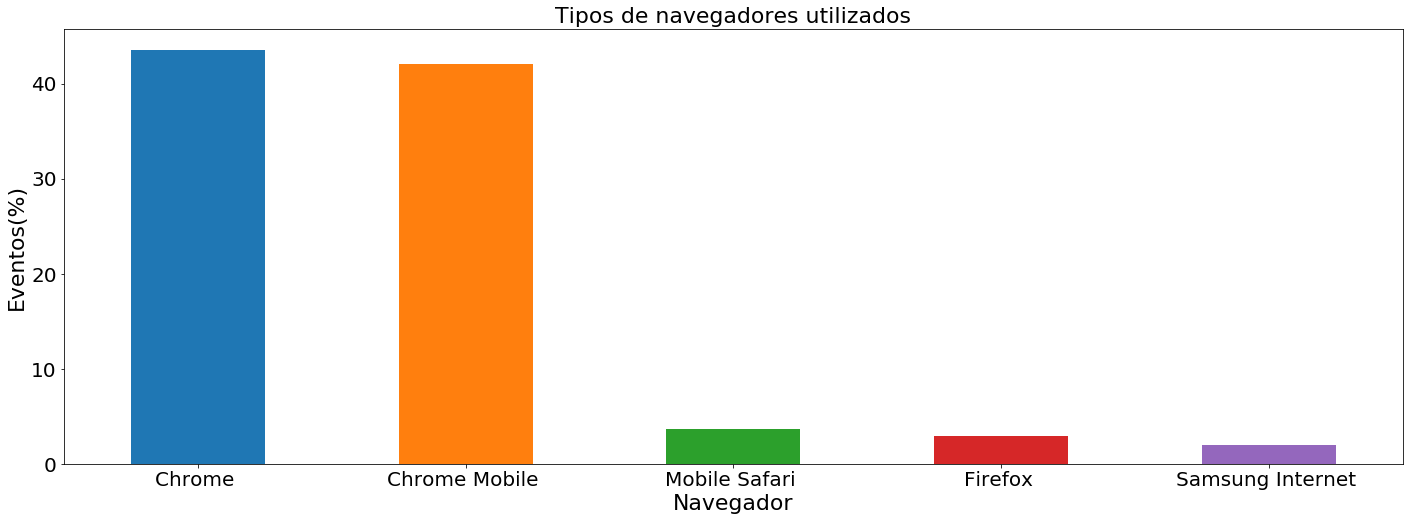
\includegraphics[width=1.1\linewidth]{output_83_1}
	Figura 25.
	
\end{center}

Es clara la supremacía de Chrome frente a otros navegadores, esto podría deberse a la inmensa cantidad de dispositivos Android que cuentan con dicho navegador como predeterminado, y su vinculación directa con el buscador de Google.\\


\newpage
\subsection{Proporción de usuarios que ingresan por un buscador }
Otro aspecto relacionado con los navegadores es la proporción de usuarios que ingresan mediante un buscador.\\


En el caso del set de datos se calculó que el 5\% de los usuarios ingresa mediante un buscador, lo que puede significar en parte a usuarios redireccionados mediante publicidades u otros sitios web.

\subsection{Buscadores más utilizados}


Teniendo en cuenta los buscadores utilizados, se observa:

\begin{center}
	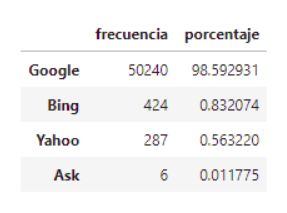
\includegraphics[width=0.5\linewidth]{table_5}
	\\Tabla 5: Buscadores más utilizados.
	
\end{center}


Esto nos permite concluir que la elección del Navegador está íntimamente relacionada con el buscador, teniendo a Google como el buscador predeterminado tanto de Chrome como de Chrome Mobile.

\newpage

\section{Análisis Geográfico}


A continuación se realizará un analisis de la distribucion geográfica de los usuarios y los eventos generados por ellos, tanto a nivel de ciudad como de pais. 

\subsection{Ciudades con más usuarios}

\begin{center}
	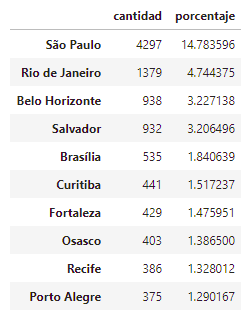
\includegraphics[width=0.5\linewidth]{table_6}
	\\Tabla 6:Ciudades con más usuarios.
	
\end{center}

\subsection{Ciudades con más eventos}

\begin{center}
	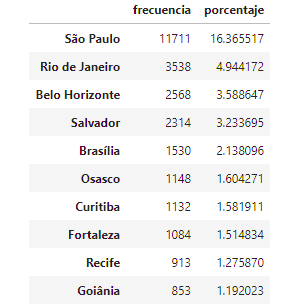
\includegraphics[width=0.5\linewidth]{table_7}
	\\Tabla 7: Ciudades con más eventos.
	
\end{center}

\begin{center}
	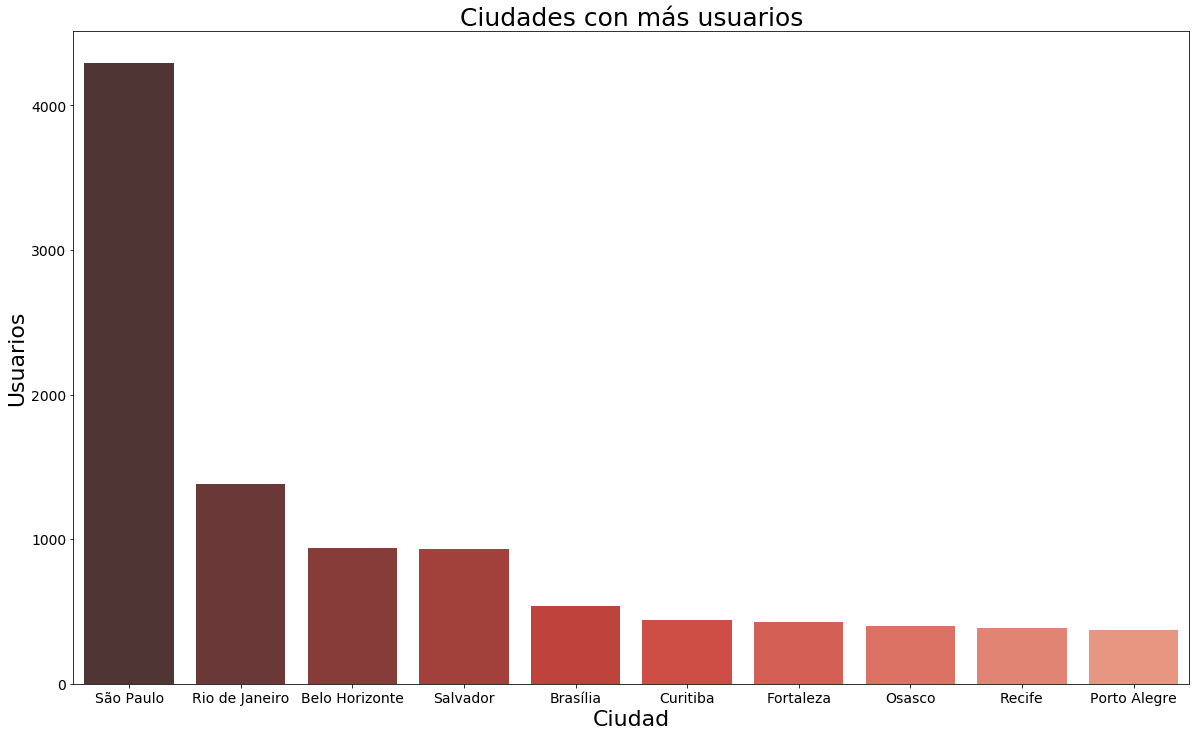
\includegraphics[width=1.1\linewidth]{output_95_0}
	Figura 26
	
\end{center}
\begin{center}
	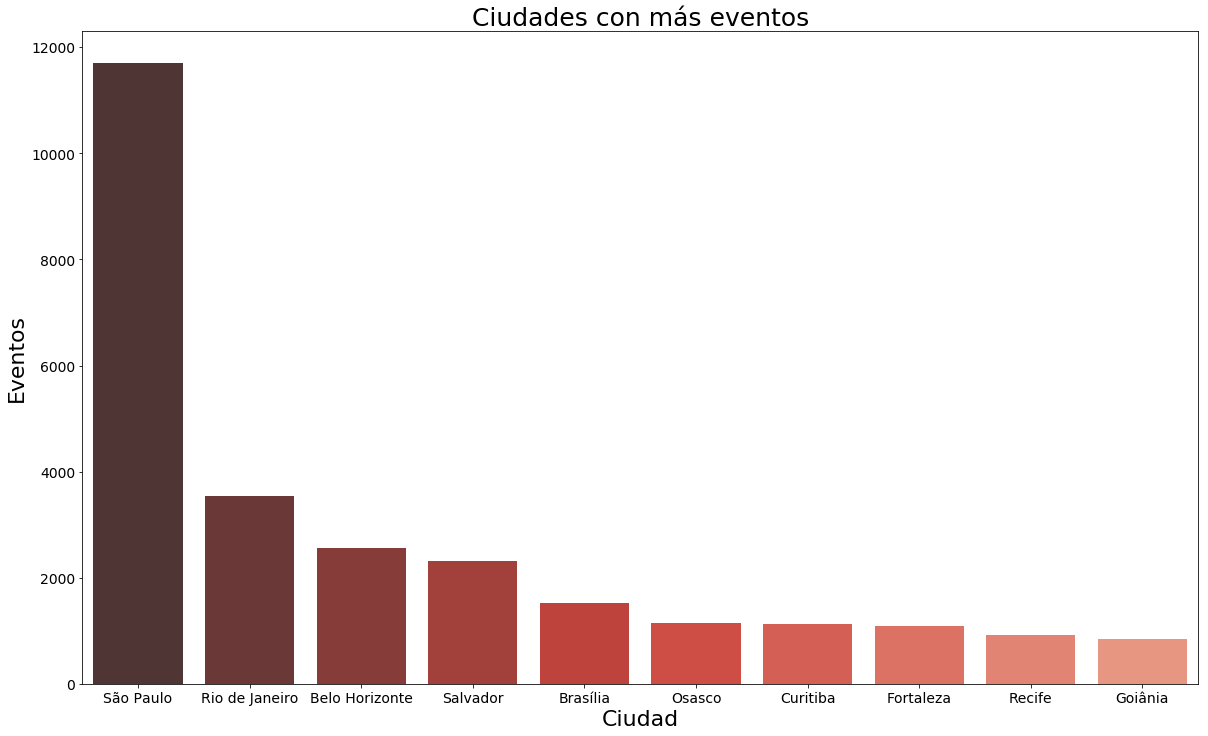
\includegraphics[width=1.1\linewidth]{output_97_0}
	Figura 27
	
\end{center}
Tanto si tenemos en cuenta la cantidad de usuarios como la cantidad de eventos, se destacan las ciudades más importantes de Brasil: San Pablo, Rio de Janeiro, Belo Horizonte, Salvador, Brasilia, etc. Es esperable la correlación entre cantidad de usuarios y cantidad de eventos por ciudad, no se detectan anomalias, por lo que se puede decir que no hay clientes que destaquen por sus volumenes de compra.

\newpage

\subsection{Países con más usuarios}

\begin{center}
	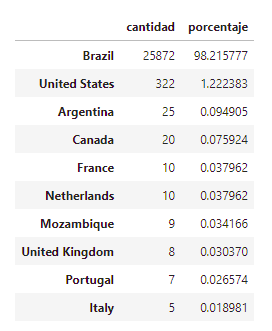
\includegraphics[width=0.5\linewidth]{table_8}
	\\Tabla 5: Países con más usuarios.
	
\end{center}

La mayoría de los usuarios son de Brasil, el porcentaje del resto de los países es depreciable frente a este.

\subsection{Países con más eventos}

\begin{center}
	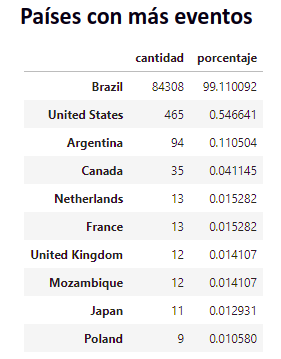
\includegraphics[width=0.5\linewidth]{table_9}
	\\Tabla 5: Países con más eventos.
	
\end{center}

\newpage
Presentamos un mapa con las visitas a la plataforma:

\begin{center}
	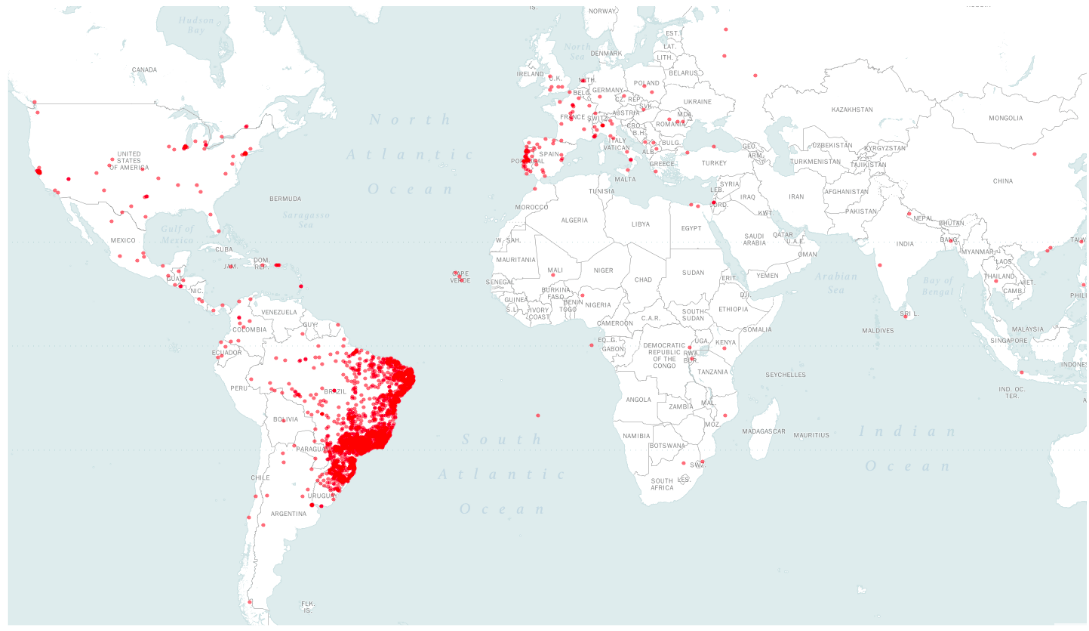
\includegraphics[width=1.2\linewidth]{map_1}
	\\Mapa 1: Mundo.
	
\end{center}

Se observan visitas aisladas de todo el mundo, pero claramente se concentran en el este de Brasil. También es destacable EEUU, distribuido en varias ciudades, Buenos Aires en Argentina, y zonas de la península Iberica.\\

Se nota muchisima actividad en las zonas de habla portuguesa e hispana, que son los dos idiomas en los que esta disponible la pagina. Seguramente \textbf{sería beneficioso contar con un sitio traducido al ingles para seguirse expandiendo por Estados Unidos}.\\

\newpage
Se presenta un mapa de Brasil con las visitas al sitio:

\begin{center}
	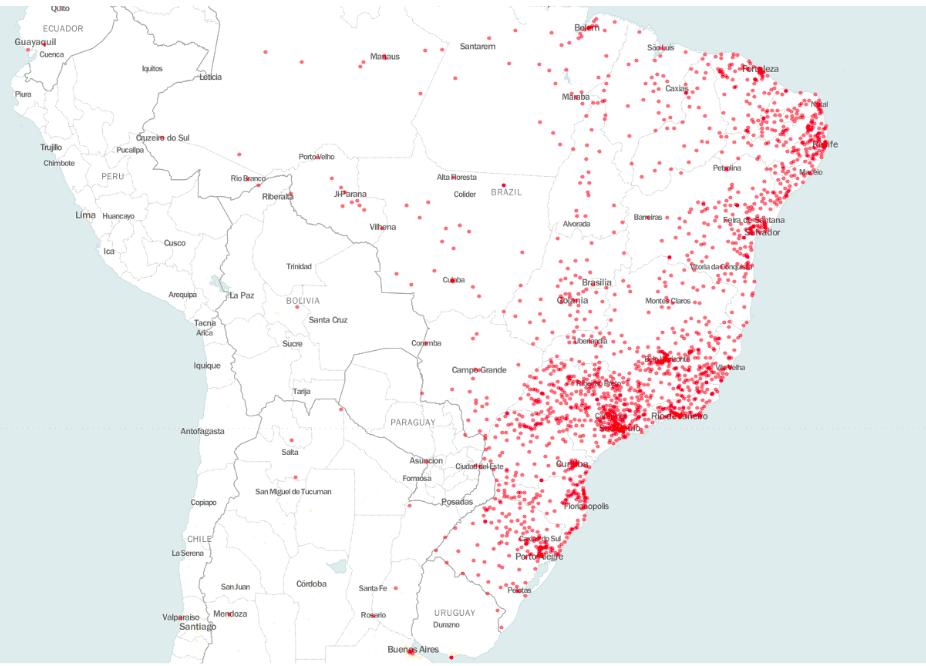
\includegraphics[width=1.1\linewidth]{map_2}
	\\Mapa 2: Brasil.
	
\end{center}

Si nos enfocamos en Brasil propiamente dicho, se puede ver que los usuarios estan bien distribuidos por todas las zonas pobladas del país, concentrandose especialmente en los principales centros urbanos.

\newpage
\section{Análisis del usuario}

Se muestran algunas cifras referidas a la actividad de los usuarios:\\

\begin{itemize}
	\item \textbf{Cantidad de personas que compraron}:
	716
	
	\item
\textbf{	Promedio de visitas de personas que compran}:
	1.6368715083798884
	
	\item
	\textbf{Máximo de compras de una persona}:
	15
\end{itemize}

\begin{center}
	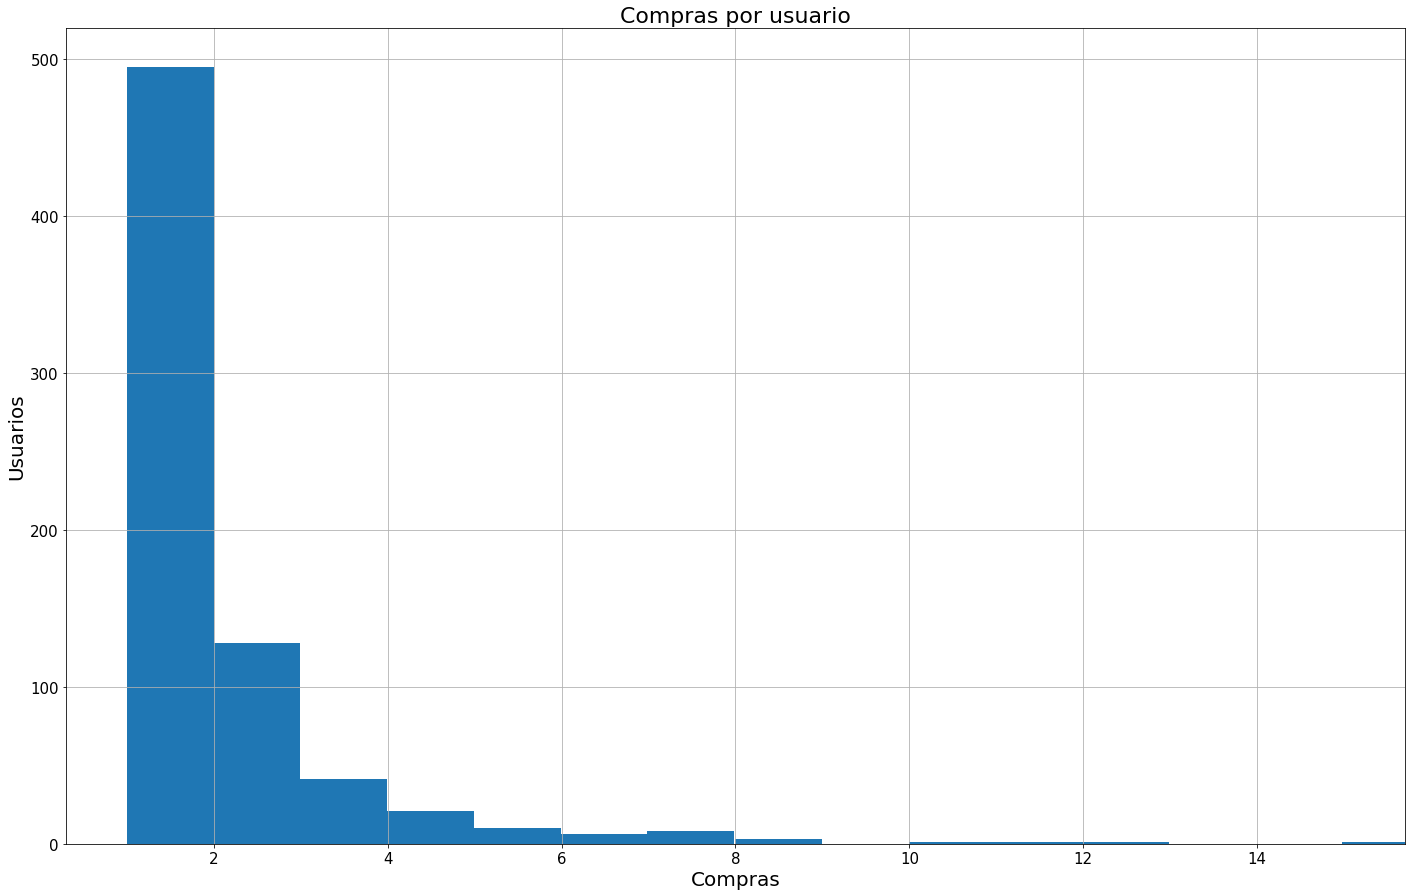
\includegraphics[width=1.1\linewidth]{output_110_1}
	\\Figura 28.
	
\end{center}


En este histograma se observa que la mayoria de las personas compras una sola vez, poco más de 100 compraron 2 veces, y a partir de ahí son valores muy bajos, aunque curiosamente un cliente realizó 15 compras.\\

\textbf{Porcentaje de usuarios que realizaron solo una compra}:
69.1340782122905
\\


\textbf{Cantidad de personas que realizaron ckeckouts}:
27624\\


Podemos ver algo interesante, porque si se calcula la cantidad de usuarios distintos, resulta ser 27624. Esto nos indica que el sistema reconoce a usuarios como distintos recién después de hacer un checkout. Esto es muy importante para entender mejor el sitema de web analytics.\\


\textbf{Promedio de checkouts por persona}:
1.22122067767159 
\\

\textbf{Relación entre personas que hicieron checkouts y personas que compraron}
2.591949029829134\\

 
Esto demuestra que mucha gente realizó un checkout, pero solo el 2,5 \% efectivamente compraron un celular.\\

\textbf{Relación entre total de checkouts y total de compras}
3.4741366533274047
\newpage
\subsection{Cantidad de productos vistos por persona}

\begin{center}
	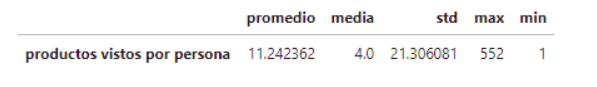
\includegraphics[width=0.9\linewidth]{table_10}\\
	Tabla 10: Cantidad de productos vistos por persona
	
\end{center}

\textbf{Usuarios que ingresan por una campaña publicitaria}:
8.190248475211808

\begin{center}
	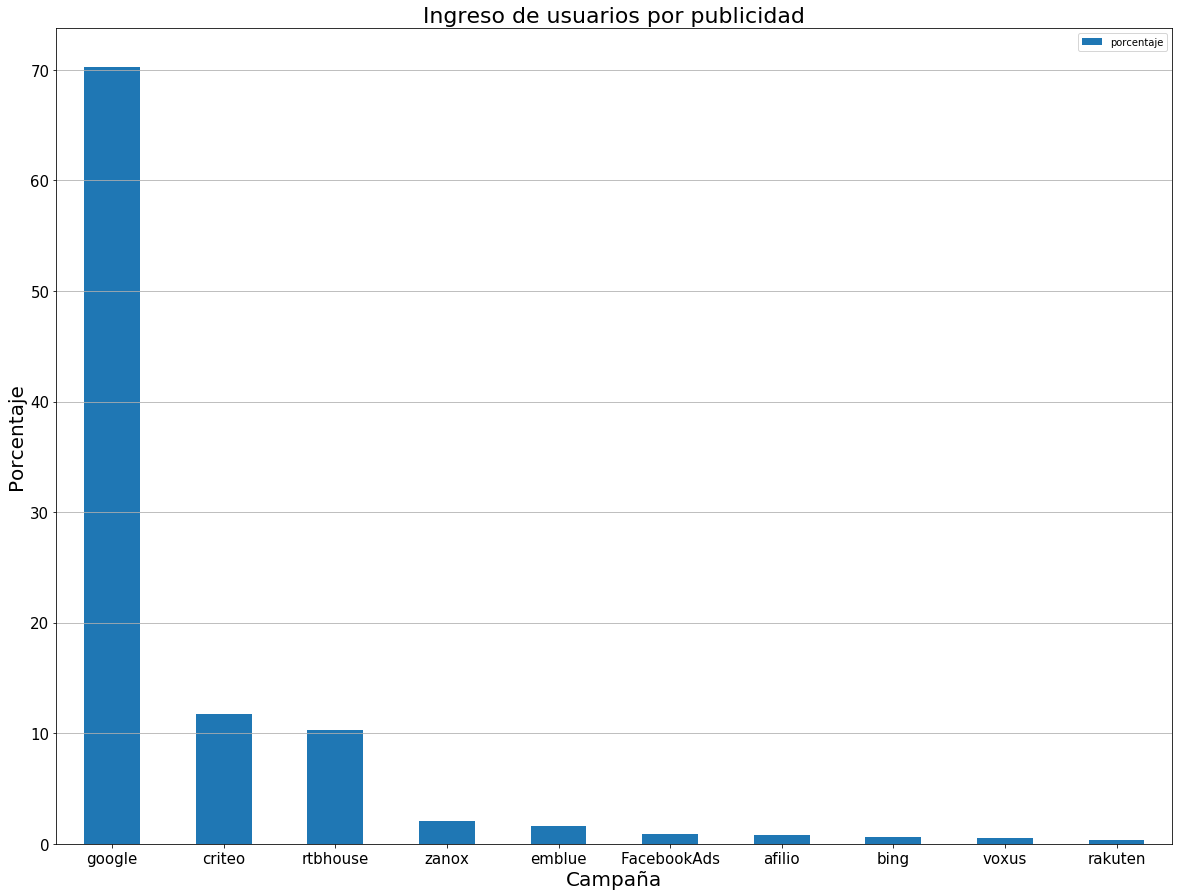
\includegraphics[width=1.1\linewidth]{output_127_0}
	Figura 28.
	
\end{center}


Como vimos anteriormente, Google es el principal buscador usado, y por lo tanto tiene sentido que la mayoría de las campañas publicitarias provengan de ahí. Es de notar que las campañas en Facebook no están resultando.
\newpage
\section{Conclusiones generales}

Al finalizar el presente trabajo, nos propusimos destacar ciertos aspectos del mismo, de tal modo que permitan a la empresa tener una visión más clara de su progreso.\\


\underline{Los principales puntos a tratar son}:

\begin{itemize}
	
\item Las ventas de celulares vienen aumentando con los meses, pero lentamente, aproximadamente 50 ventas más por mes.

\item Las campañas y avisos publicitarios deben publicarse durante la semana, y no en el fin de semana.
Además, dichas campañas deben mostrarse a partir de las 16:00, recordando que la mayor actividad ocurre a la noche.

\item El día martes es un buen candidato para publicitar, tal vez porque los lunes son muy cargados de trabajo, y recién el martes uno tiene más libertad.

\item Continuar con la campaña de subscripciones, luego de realizar una compra, pues en el último mes viene dando resultados.

\item Si bien la marca más comprada es Samsung, deberían profundizar en la venta de iPhone, que son los más visitados, pues están de moda por ser considerados de alta gama. Esto no implica no seguir con los modelos de Samsung, simplemente abrir el panorama.

\item Si bien los celulares de 16gb son los más vendidos, prestar atención con los de 32gb, que podrían ser los próximos protagonistas. A aquellos con 8gb, no brindar tanto soporte como antes.

\item La condición “Bueno” sigue siendo la más visitada y comprada, tener esto en cuenta.
Cada mes más usuarios compraron a partir de una campaña, pero como se vió en el análisis, la unica con resultados significativos es la de Google. Por lo tanto, creemos que que debería continuarse con esta modalidad, pero habría que evaluar la relación costo beneficio de las otras campañas publicitarias.

\item Dar soporte especializado al navegador Google Chrome, tanto en su versión de escritorio como en su versión mobile, los otros no son tan significativos a nivel cantidad de usuarios.

\item Por su parte, las tablets están en desuso, por lo tanto, enfocarse en los smartphones principalmente, que van a superar las computadoras de escritorio pronto, en términos de uso.

\item Si bien la mayoría de los usuarios son de Brasil, se noto una creciente actividad en los Estados Unidos. Por lo tanto, una propuesta es traducir la página web al inglés, para promover la visita de personas de dicho país. También notamos un posible negocio futuro en Argentina, donde se debe hacer hincapié en la diferencia de precio con respecto a otros vendedores.  

\item Por último, se debe volver a hacer un análisis de datos en unos meses, y verificar el progreso de la empresa en base a las recomendaciones propuestas, para determinar el correcto camino.

\end{itemize}


\newpage



\begin{thebibliography}{99}
		
	\bibitem{}Trocafone website, \url{www.trocafone.com}.
	
	\bibitem{} NumPy - NumPy, \url{http://www.numpy.org/}.
	
	\bibitem{} Python Data Analysis Library,
	\url{https://pandas.pydata.org/}.
	
	\bibitem{}	Matplotlib: Python plotting — Matplotlib 3.0.0 documentation,
	\url{matplotlib.org}.
	
	
	\bibitem{}seaborn: statistical data visualization — seaborn 0.9.0 documentation,
	\url{seaborn.pydata.org}
	
	\bibitem{} Folium information,
	
	\url{https://github.com/python-visualization/folium}
	
	\bibitem{} GeoPy’s documentation,
	
	\url{
	https://geopy.readthedocs.io/en/stable/}
\end{thebibliography}


\end{document}
